%%%%%%%%%%%%%%%%%%%%%%% file template.tex %%%%%%%%%%%%%%%%%%%%%%%%%
%
% This is a template file for the LaTeX package SVJour2 for the
% Springer journal "Biological Cybernetics"
%
%                                    Springer Heidelberg 2004/11/R22
%
% Copy it to a new file with a new name and use it as the basis
% for your article
%
%%%%%%%%%%%%%%%%%%%%%%%%%%%%%%%%%%%%%%%%%%%%%%%%%%%%%%%%%%%%%%%%%%%
%
% First comes an example EPS file -- just ignore it and
% proceed on the \documentclass line
% your LaTeX will extract the file if required
\begin{filecontents*}{example.eps}
%!PS-Adobe-3.0 EPSF-3.0
n%%BoundingBox: 19 19 221 221
%%CreationDate: Mon Sep 29 1997
%%Creator: programmed by hand (JK)
%%EndComments
gsave
newpath
  20 20 moveto
  20 220 lineto
  220 220 lineto
  220 20 lineto
closepath
2 setlinewidth
gsave
  .4 setgray fill
grestore
stroke
grestore
\end{filecontents*}
%
\documentclass[twocolumn,fleqn]{svjour3}
% Biological Cybernetics uses author year
% references, hence the natbib package is activated - use
% \citet{...} and \citep{...} with it to cite references.
%
\smartqed  % flush right qed marks, e.g. at end of proof
%
\usepackage[numbers]{natbib}
\usepackage{amssymb}
\usepackage{amsmath}
\usepackage{textcomp}
\usepackage[T1]{fontenc}
\usepackage[utf8]{inputenc}
\usepackage[english, spanish]{babel}
\usepackage{csquotes}
\usepackage{enumerate}
\usepackage{enumitem}
\usepackage{caption}
\captionsetup{compatibility=false}
\usepackage{subcaption}
\usepackage{listings}
% para la lista de simbolos
\usepackage{array} %for vertical thick lines in tables
\usepackage{multirow} %multirow tables
\usepackage{nicefrac} %for fractions like 1/4
\usepackage[dvipsnames]{xcolor}
\usepackage{pgfplots}
\pgfplotsset{compat=default}
\usepackage{pgfplotstable}
\usepgfplotslibrary{statistics}
\usetikzlibrary{spy}
\usepackage{longtable}
\usepackage{array}
\usepackage{pdflscape}
\usepackage{booktabs}
\usepackage{graphicx} % figuras
%\usepackage{subfigure} % subfiguras



%
% \usepackage{mathptmx}      % use Times fonts if available on your TeX system
%
% insert here the call for the packages your document requires
%\usepackage{latexsym}
% etc.
%
% please place your own definitions here and don't use \def but
% \newcommand{}{}
%
\journalname{}

\DeclareUnicodeCharacter{2217}{*}

\begin{document}

%\title{Ordenamiento de colores RGB basado en m\'etricas asociadas a la imagen}
\title{RBG ordering based on image metrics}
\author{
  Jos\'e Luis V\'azquez Noguera \and
  Christian E. Schaerer \and
  Jacques Facon	\and
  Horacio Legal Ayala
}

\institute{
  Jos\'e Luis V\'azquez Noguera  $\cdot$ Horacio Legal Ayala $\cdot$ Christian E. Schaerer \at  
  Polytechnic Faculty, National University of Asuncion - San Lorenzo, Paraguay \\
  \email{\{jlvazquez,hlegal,cschaer\}@pol.una.py}  
  \and
  Jacques Facon \at
  PPGIa - PUCPR-Pontifícia Universidade Catolica do Paraná - Curitiba - Pr, Brazil \\
  \email{facon@ppgia.pucpr.br}  
}

\date{Received: date / Revised: date}
% The correct dates will be entered by the editor
\maketitle

\begin{abstract}
  In color ordering literature, the lexicographical ordering and its variants are the most used methods and an usual problem is the ``a priori'' definition of the most important color component \textbf{(NE...)}
  This paper proposes a new ordering criteria, which assign a weight to every component in accordance with the metrics applied to it, with this criteria we pursue to avoid arbitrary definitions and build the ordering based on image-based information. \textbf{... Obtener los terminos correctos de fuentes oficiales (filtrado de imagenes, mejora de constraste...)}
  Applications used for validation of the proposal are: image filtering, contrast improvement and textures characterization for later classification. The results using the proposed ordering in different applications are better in most cases compared to different ordering methods of the state of the art.
\end{abstract}

%\section{Introducci\'on}
\section{Introduction}
\label{intro}

Digital image processing on color images resemble human vision \cite{roerdink2000watershed}, which is \textbf{NE...}, on the other hand grayscale images and binary images contribute less information because of their use of single dimentional intensities and binary values, white and black. At its inception, digital image processing algorithms where only develop for grayscale and binary images because of the limited computing power available at the time and their high cost, these conditions demands to reduce the visual information into a single plane.
\textbf{ver citas en inglés...}


Valuable information can be obtain from grayscale images, for example an object boundaries could been detected from sudden changes in intensities. By calculating the gradient \textbf{on every pixel (Added)} we could extract every object from the image, however unexpected reflections could produce errors on the boundaries detections. Reflections, lighting effects and the lack of chromatic information limit the efficiency of many grayscale algorithms \cite{ortiz2002procesamiento}. Considering these ideas and the new improvements on computational resources, as image processing specialized processors \textbf{review}, a lot of grayscale images are been generalized into color images \cite{ortiz2002procesamiento}.
  

Color spaces are formalisms \textbf{(alternative)} that allow the definition of color and their properties for proper manipulation \cite{joblove1978colo,meyer1980perceptual}.


The most used color space on screens is the RGB color space, which it is based on the tristimulus model and aditive syntesis of color \textbf{review from cite}. In the RBG color space a color, where the colors used are red, green and blue, is defined as 3-tuples where the scalar value on every component measures its influence on the mix \cite{tkalcic2003colour}. In the CMY color space, cyan, magenta and yellow also known as secondary colors, represents the substractive syntesis of color \cite{rolleston1996color}. The CMYK color space, used in printers\cite{rolleston1996color}, extends the previous color space adding the K component which represents the maximum value between the 3 secondary values\cite{tkalcic2003colour} \textbf{NE}.


The XYZ color space has been introduced because there are some colors that can only be represented by a negative value of stimuli \textbf{review} and it is a linear transformation over the RGB color space\cite{ortiz2002procesamiento}. This color space is used when the color representation is independent of the hardware.


The L*a*b* is a 3 component color space where the L* represents the luminosity from black to white, the a* measures from red to green and the b* from yellow to blue\cite{leon2006color} \textbf{review from cites}.


The color spaces HSI, HLS, HSV and their variants are the color spaces that resembles the human vision the most because they are based on luminosity, saturation and hue perseptions\cite{zamora2001comparativos}.


A lot of aplications needs color ordering, as noise reduction, contrast enhancement, borders detection and segmentation of color images\textbf{review terminos}\cite{ortiz2002procesamiento}. Because of \textit{multi}-dimentional nature of color representation their is no natural order and \textbf{NE}.


This work presents a new ordering for the RBG color space based on the metrics associated to each component. The proposed ordering is compared with the state of art orderings on noise reduction, contrast enhancement and texture characterization. \textbf{IMP REVIEW}


The paper is organized as follows. The second section presents the current state of the art on the matter. The third section presents the fundamentas of color image filtering as main conceps of image filtering, ordering and mathematics morphology. The fourth section presents the proposed ordering. The fifth section presents the experimental results of the comparisons with the current state of the art on aplications as noise reduction, contrast enhancement and texture characterization. Finally, the sixth and last section presents our conclutions for future works.\textbf{review}.

\section{State of the art \textbf{methods.??}}
\label{Relacionados}

The extension of the filter order to color images requires on the one hand select the color space in which the image is processed and in the other establish an order in this color space. To establish an arrangement they have worked in different color spaces, among which we can mention, L*a*b* color spaces \cite{hanbury2001mathematical}, HLS \cite{hanbury2001mathematical2},  CIELAB \cite{hanbury2002mathematical3}, HSI \cite{tobar2007mathematical}, HSV \cite{lei2013vector} and the RGB color space  \cite{zaharescu2003color, gao2013adaptive, wang2012edge}.

\textbf{....}


Mathematical morphology borns in 1964 from the colaboration of Georges Matheron and Jean Serra at École de Mines, Paris \cite{serra1982image} and currently ir reach is as broad as image processing itself. A few examples of aplications are image segmentation, restoration, border detections, contrast enhacement, texture analysis, compression, etc. \cite{ortiz2002procesamiento}.
Erosion and dilation are the most basic operations where \textbf{NE reticulo?}\cite{heijmans1990algebraic}. Erosion is the minimum and dilation is the maximum of a window \textbf{review for better terminology} called structural element and from this two all other operations are builded. To generalize the mathematical morphology to color images is required an ordering between colors to be able to determine a minimum and a maximum inside the structural element.


Recent publications presented generalizations of mathematical morphology \cite{ledoux2012limits, van2013group, velasco2012random, lezoray2009learning, velasco2010morphological, burgeth2013morphology, velasco2011supervised, hanbury2001morphological, angulo2010pseudo, aptoula2008alpha, kleefeld2015processing, vazquez2014color}. In RGB the interlace bit ordering \textbf{review...!!} has been proved to be efficient on color image filtering \cite{chanussot1997bit}. For a more in depth analysis on mathematical morphology methods, we suggest Aptoula and Lefevre \cite{apatoula2007comparative}.

%El art\'iculo \cite{aptoula2007comparative} incluye m\'as de 70 referencias distintas de m\'etodos de morfolog\'ia matem\'atica a color, mostrando as\'i, aparte de una revisi\'on del estado del arte, que el \'area es reciente. Se han propuesto una gran cantidad de m\'etodos para realizar la extensi\'on de morfolog\'ia matem\'atica a color; entre los art\'iculos recientes podemos citar \cite{ledoux2012limits, van2013group, velasco2012random, lezoray2009learning, velasco2010morphological, burgeth2013morphology, velasco2011supervised, hanbury2001morphological, angulo2010pseudo, aptoula2008alpha, kleefeld2015processing, vazquez2014color}. 


Generally, that is for many color spaces, the lexicographical arrangement is one of the most used in the literature \cite{aptoula2007comparative, aptoula2008lexicographical}, since it has desired theoretical properties and can easily customize the way you are going to compare the components of the image. 


Louverdis et. al. \cite{louverdis2002new} and Vardavoulia et. al. \cite{vardavoulia2002vector} presents a lexicographic ordering in HSV, while Louverdis et. al. \cite{louverdis2002morphological} uses the same ordering and color space to develop a novel morphologic method for shape and size analisys on granular images. Angulo and Serra \cite{angulo2003morphological} discuss over lexicographic ordering on RGB and HLS for JPEG image compression. Ortiz et. al. \cite{ortiz2004morphological} uses the I→H→S $(Href=0º)$ lexicographical ordering for gaussian noise elimination.

%Un ejemplo de ordenamiento lexicogr\'afico en el espacio de color HSV se puede encontrar en \cite{louverdis2002new}, mientras que \cite{louverdis2002morphological} y } utilizan el mismo orden, respectivamente, para el filtro de la mediana y el c\'alculo de granulometr\'ia en im\'agenes a color. Por supuesto, tambi\'en puede haber situaciones espec\'ificas donde la informaci\'on crom\'atica es m\'as significativa, por ejemplo, en \cite{ortiz2002colour} la matiz se compara por primera vez en la cascada lexicogr\'afica.  En \cite{ortiz2004gaussian} la eliminaci\'on de ruido se consigue por medio del ordenamiento lexicogr\'afico en el espacio HSI, utilizando la intensidad en la primera posici\'on en la cascada lexicogr\'afica. El espacio L*a*b* \cite{hanbury2002mathematical3} ha sido tambi\'en utilizado con un ordenamiento lexicogr\'afico. Por otra parte, un estudio a fondo del potencial de este orden en el espacio HLS se proporciona en \cite{hanbury2001mathematical2}, mientras que en \cite{angulo2003mathematical} el uso del ordenamiento lexicogr\'afico en el espacio HLS mejorado (IHLS) ha sido explorado.


The lexicographical ordering suffers from a serious inconvinient. More precisely, the final result of most lexicographical ordering are highly biased towards the first components where the last components are virtually ignored \cite{hanbury2002mathematical3} \textbf{over reaction?}.
 
In order to improve the tuning degree of influence of each component of the vector in the comparison result they were proposed variations lexicographic ordering. A group of variants is based on the use of an additional component for comparison.


Angulo \cite{angulo2005morphological} and  Sartor et. al. \cite{sartor2001morphological} located in the first position of the lexicographical cascade a distance measurement to a reference vector. Comer et. al. \cite{comer1999morphological} used a Euclidean norm as a method of sorting pixels, i.e. the reference pixel color is the black (0,0,0) in RGB.Two RGB colors can be visually practically identical but differ in value standard, or distance to a reference color, as well as two different colors have the same norm so it is not recommended to use this strategy. In the L*a*b space there is a defined distance measure, about the origin $L=0$, $a=0$ and $b=0$ which it is widely used for the evaluation of the quality of reproduction in color, or in techniques of understanding of color images. \cite{tremeau1998analyse}.   

Other types of arrangement seeking the extension of lexicographic ordering is to use a parameter $\alpha$  defined by the user so as to modify the degree of influence of the first componente \cite{ortiz2002procesamiento,angulo2005unified}. Even with the changes in the lexicographic ordering, the criteria for choosing which component will have higher priority in the comparison, and the value $\alpha$ are usually arbitrary. Gao et. al. \cite{gao2013adaptive} tries to solve this problem by presenting an approach of adaptive lexicographic ordering. 
In order to avoid the most subjective user intervention, it would be of great importance that the arbitrary criteria of lexicographic order and its variants can be eliminated or reduced.


Bouchet et. to the. \Cite{bouchet2016fuzzy} uses fuzzy logic so that the three color components have the same weighting in the sorting, although it is desirable that the priority of the components of the vector representing the image are audited self-image information, not being exactly the same in all cases. Benavent et. al. \cite{benavent2012mathematical} presents a sorting method that is dependent of the image and ordering the colors according to the probability density of the appearance of colors in the image.

The main difference of this proposal, with those presented in the state of art, is the extraction of information for each component of RGB color in a specific domain image. This information is extracted by a vector of weights which are previously calculated by a function applied to each of the RGB components of the color.



\section{Fundamentals of color image filtering}
\label{Teo}

This section presents the formal formulations of the theoretical concepts behind the extension order filters for color images, vector arrangement and morphological mathematics.

\subsection{RGB images}

In general, an image is a function $f:\mathbb{Z}^2 \rightarrow \mathbb{Z}^n$. Ech pair $(u,v) \in \mathbb{Z}^2$ is a pixel, and $f(u,v) \in \mathbb Z^n $ is the color image in the pixel $(u,v)$. In particular, a RGB image (red, green and blue) with a color depth of k bits is, $f(u,v) = (R,G,B)$, where $R,G,B \in \{0,1,...,2^k-1\}$ is the intensity of the component and $f(u,v)$ is the color resulting from mixing these components in the pixel $(u,v)$. %Si el vector $\mathbb Z^3$ es una tripleta correspondiente a los componenetes rojo, verde y azul, la imagen $f$ es llamada imagen  RGB.
The image $f$ can digitally presented as an array $M \times N \times 3$ , where each pixel $(u,v)$ has as its value a triplet $(R,G,B)$ \cite{gonzales2004digital}. An RGB image can be seen as a ``stack'' of three images in grayscale (see Figure \ref{fig:ImagenRGB}) that, when fed to the red, green and blue entries of the color monitor, produces a color image on the screen \cite{gonzales2004digital}.


\begin{figure}[htbp]
	\centering
		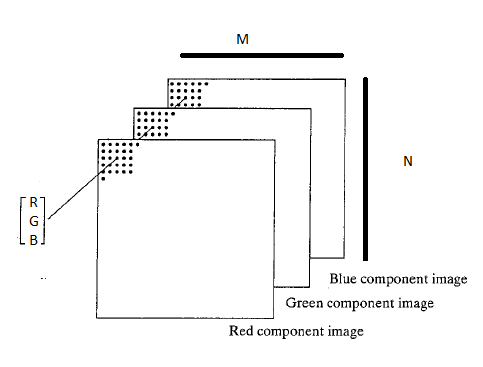
\includegraphics[scale=0.65]{fig/ImagenRGB.png}
	\caption{RGB Image}
	\label{fig:ImagenRGB}
\end{figure}

%\subsection{Histogramas}


%\subsubsection{Histograma de color}
%El histograma a color  de una imagen $f $ en un dominio $D$  es una función discreta definida como sigue:
	
%	\begin{equation}
%	\label{eq:histograma_color}
%	H^D_{f}(C) = n_C,
%	\end{equation} donde  $C = (C_1, C_2, C_3)$, $C_i \in \{0, ..., 2^k - 1\}$ y $n_C$ es la cantidad de veces que aparece el color $C$ en el dominio $D$ de la imagen $f$. 
	
%	Etiquetemos a cada color dentro del espacio discreto con los superíndices $a$  y $b$. El color $C^a$  es menor al color $C^b$ si $C^a_1 < C^b_1$, $C^a_2 < C^b_2$ y  $C^a_3 < C^b_3$. 
	
%	El objetivo es fijar un orden de colores en el espacio de color discreto, normalmente utilizando el orden natural ascendente (Cuadro \ref{table:orden_color}).
	
%	\begin{table}[!htpb]
%		\centering
%		\caption{Orden natural de colores}
%		\label{table:orden_color}
%		\begin{tabular}{|c|c|}
%			\hline
%			$a$   & $C^a$                                                                     \\ \hline

%			0   & (0, 0, 0)                                                             \\ \hline
%			1   & (0, 0, 1)                                                             \\ \hline
%			2   & (0, 0, 2)                                                             \\ \hline
%			3   & (0, 0, 3)                                                             \\ \hline
%			\vdots & \vdots                                                                      \\ \hline
%			$2^{3k}-2$ & ($2^k-2$, $2^k-2$, $2^k-2$) \\ \hline
%			$2^{3k}-1$   & ($2^k-1$, $2^k-1$, $2^k-1$) \\ \hline
%		\end{tabular}
%	\end{table}

%	El histograma de color acumulado $\bar{H}^D_f$ de la imagen $f$ un dominio $D$ es definido en términos del histograma a color $H^D_{f}$: 
	
%	\begin{equation}
%	\bar{H}^D_f(C^b) = \sum_{C^a \leq C^b} H^D_f(C^a)
%	\end{equation}




\subsection{Image filtering}
Image filtering covering all techniques in the processing of images, that from an input image, another image is obtained in which is remove, emphasize or highlight some features of the input image. 
A filter $F$ of a digital image color $f$ can be expressed as:

\begin{equation}
\label{Filtrado} 
      g(u,v) = F\{f(u,v)\}
\end{equation}
where $f(u,v)$ is a color of the input image, $g(u,v)$ is a color of the image output and $F$ is the filter defined over a window of the pixel $(u,v)$.


Order filters are operations nonlinear neighborhood, where a function is applied to each pixel neighborhood. The idea is to move a window centered on the pixel, either a rectangle (usually a rectangle of odd sides) or other shape on an image given. By doing this, we create a new image whose pixels are the result of obtaining a value of the color under the mask presorted (Figure \ref{fig:Filt}). 


\begin{figure}[htbp]
	\centering
		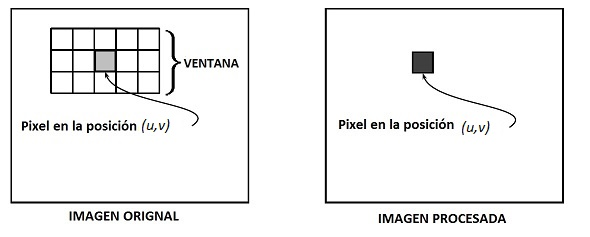
\includegraphics[scale=0.5]{fig/Filt.jpg}
	\caption{Digital image filtering.}
	\label{fig:Filt}
\end{figure}



For example, a pixel of the new image can be a result of obtaining the median, minimum or maximum of the colors arranged in the window of the processed image.  
The combination of the window and the function is called filter. 

\subsection{Sorting}
The concept of order plays a important role to use a filter order, or to define the basic operations of mathematical morphology. For a thorough study of the theory of order the reader can see \cite {serra1993anamorphoses}.

%Una relaci\'on binaria $\leq$ en un dominio $D$ se llama:

%\begin{enumerate}
%\item \label{reflexiva} reflexiva si $C\leq C'$, $\forall C\in D$		 
%\item \label{antisimetrica} antisim\'etrica si $C \leq C' \wedge C' \leq C$\,$\Rightarrow$ \, $C=C'$,  $\forall C,C'\in D$
%\item \label{transitiva} transitiva si $C \leq C'$ $\wedge$ $C' \leq C''$\,$\Rightarrow$ \, $C \leq C''$,  $\forall C,C',C''\in D$
%\item \label{total} total si $C' \leq C$ $\vee$ $C' \leq C$,  $\forall C,C'\in D$
%\end{enumerate}
%Una relaci\'on binaria $\leq$ es llamada de \emph{pre-orden} si cumple con \ref{reflexiva} y \ref{transitiva}; si a su vez cumple con \ref{antisimetrica} se convierte en una relaci\'on de \emph{orden}. Si adicionalmente cumple con \ref{total}, es denotada como \emph{total}, si no lo hace como \emph{parcial}.
  
%La estructura en un espacio de color est\'a dada por un ret\'iculo completo. Un ret\'iculo completo ${\cal L}$ es un conjunto no vac\'io con orden parcial  ${\cal R} $ tal que cualquier subconjunto no vac\'io  ${\cal P}$ de  ${\cal L}$ tiene un \'infimo  y tiene un supremo. 

According to the article  \cite{barnett1976ordering}, ordering vector arrangement techniques can be classified into the following groups:
\begin{itemize}
\item Marginal Sorting (M Sorting): The marginal arrangement compares each color component independently.
\item Conditional Sorting (C Sorting ): The vectors are sorted by some marginal component selected sequentially according to different conditions. The lexicographic order is a well-known example of C Sorting  employing all available components of the given vectors.
\item Partial Sorting (P Sorting): This ordering is based on the partition of the vectors in groups of equivalence such that  between groups there exist an order. In this case, "partial'' is an abuse of terminology, as there are total ordering that belong to this particular class. 
\item Reduced Sorting (R Sorting): The vectors are first reduced to scalar values and then classified according to their naturally scalar order. For example, a R ordering in  $\mathbb{Z}^n$ could be first define a transformation $T:\mathbb{Z}^n\rightarrow \mathbb{R}$ and then sort the colors with respect to the scalar order of his projection in $\mathbb{Z}^n$ by $T$.
\end{itemize}

In practice there are two general methods for processing color images: marginal and vectorial.

The marginal processing consists in the separate processing of each component of the image. Despite its simplicity, the marginal processing has two disadvantages \cite{aptoula2007comparative}: 
\begin{itemize}
    \item The correlation between components is completely ignored.
    \item Creates false colors after processing.
\end{itemize}

The use of marginal processing is inadequate for images with highly correlated components (eg RGB color images) \cite{astola1990vector}. Therefore this work focuses on the vectorial processing will be explained below. 

%\begin{figure}
%	\centering
%		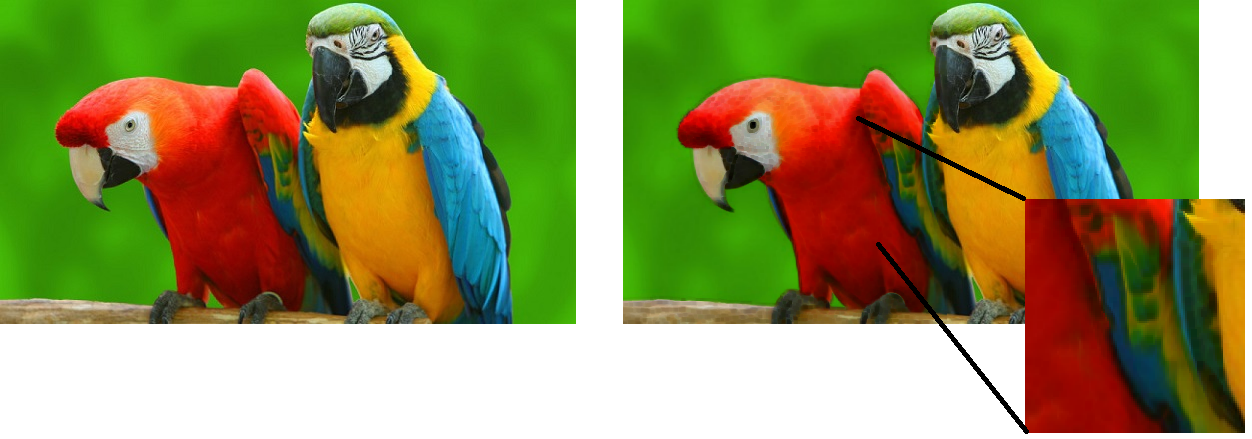
\includegraphics[scale=0.5]{fig/resultado.png}
%		\caption{Imagen original y su erosión utilizando el ordenamiento marginal. En la erosión aparecen %nuevas cromaticidades.}
%	\label{fig:resultado}
%\end{figure}

The vector processing processes all available globally and simultaneously components.
Since vectors (way representing a color) are considered as the new processing units, the correlation between the different components is no longer ignored. However, compared to its counterpart marginal, the most significant drawback of the approach vectorial is mainly the need to adapt existing algorithms in order to accommodate vectorial data \cite{aptoula2007comparative}. 


The vectorial processing can have two approaches:
 
\begin{itemize}
    \item Based on the preorder relationship .
    \item Based on the order relationship 
\end{itemize}

The approach based on relationship preorder,  is the set of approaches that do not comply the antisymmetric property.  Thus different colors can eventually become equivalent. So to resolve existing ambiguities, additional action are necessary. The main method of sorting of this approach is based on the Reduced Sorting (R Sorting ), where colors are reduced to scalar values corresponding to his norm, or the distance to a some reference color. 


The approach based on order relationship, in the same way can be partial or total. If the relationship is partial, there will be colors that they can not be compared. 

The total order relation has two main advantages. First, all colors are comparable, and second, there are no distinct colors that can be equivalent. Because of this, most works are based on approaches of total order relation. \cite{aptoula2007comparative}. In particular, the lexicographical order ( C Sorting ), along with its variants is among the most widely deployed options.  
 


\subsection{Morphological mathematics}

Mathematical morphological operations are based on two basic operators: dilatation and erosion. Both operators are filters that can be defined from the minimum and maximum within a window called structuring element \cite{serra1986introduction}. From erosion and dilation can extend all the morphological mathematics. Morphological operators must comply certain theoretically properties, such as anti-extensive or extensive, idempotent, homotopic and growing \cite{serra1986introduction}.

Given a digital image $f$ and $B$ window, called structuring element. The erosion ($\varepsilon$) and the dilation ($\delta$) of the image $f$ by $B$ can be expressed as:

\begin{equation}
\varepsilon(f,B)(u,v)  = \min_{(s,t) \in B} \{f(u-s,v-t) + B(s,t) \}
\end{equation}

\begin{equation}
\delta(f,B)(u,v)  =  \max_{(s,t) \in B} \{f(u+s,v+t) - B(s,t) \}
\end{equation}

We called $\delta(f,B)$ and $\varepsilon(f,B)$ as dilation and erosion respectively for all pixels $(u,v)$ of the image $f$. The combination of erosion and dilation produces other operators such as opening and closing. The opening softens the bright regions of the image. The closure softens the dark areas of the image. The opening $\circ$ and the closing $\bullet$ of $f$ by $B$ are defined based on dilation and erosion as follows:

\begin{equation}
f\circ B = \delta(\varepsilon(f,B),B),
\end{equation}

\begin{equation}
f\bullet B = \varepsilon(\delta(f,B),B).
\end{equation}

Based on the opening and closing is defined the top-hat transform. The clear top-hat transform ($WTH$) could extract bright regions of the image and the dark top-hat transform ( $BTH$ )
could extract dark areas . The transformed $WTH$ and $BTH$ are defined for an image $f$ as follows:

\begin{equation}
WTH(f) = f - f\circ B,
\end{equation}

\begin{equation}
BTH(f) = f\bullet B - f. 
\end{equation}

The extent of the mathematical morphological color images is still an open problem \cite{aptoula2007pseudo}, mainly by the drawback that not exist a natural order between vectors, and that colors can be represented in different ways (forming different color spaces). In the absence of a natural order between colors it is not easy to define the basic operators of erosion and dilation.  

The following section presented  an ordering strategy of RGB colors, given metric extracted from each color component, so as to establish weights to components from own image information.



 \section{Proposed Sorting}

A histogram function is defined from the RGB image, which corresponds to the frequency distribution of the values that can take a picture $f$, either in a plane or in three dimensions (R, G, B). The histogram of the j-th component of the color image $f$ (R, G o B) is a discrete function $h_{f_j}^{D}$ defined as:% $h:\{0,1,\dots,t_{max}\}\times \{C_1,C_2,\dots,C_n\}\rightarrow \mathbb N$ definida como:

\begin{equation}
\label{histograma}
   h_{f_j}^{D}(i) = n_i,
\end{equation} 
where ${i}$ represents the $i-esimo$ intensity level in the range $\{0,1,...,2^k-1\}$ 
of the component $j$, and $n_i$ is the number of pixels in the image $f$ whose intensity level is $i$ in the component $j$ 
within the domain $D$ (subset of pixels $(u,v)$ inside the image $f$).

The probability of occurrence $p_{f_j}^{D}(i)$ of each level of intensity $i$ in the component $j$ of the image $f$ in the domain $D$ is defined as:
\begin{equation}
\label{probabilidad}
   p_{f_j}^{D}(i) = \frac{h_{f_j}^{D}(i)}{n},
\end{equation} Donde $n = n_0 + n_1 + ... + n_{255}$, es decir la cantidad total de pixeles de la imagen $f$ dentro del dominio $D$. 

So to avoid giving the highest priority to a component of the vector representing the color, a new value $(R,G,B)$ in the first position of the corresponding lexicographical cascade transformation obtained from metric associated to each component is placed.
RGB colors are reduced to a scalar value. For this purpose, is first defined a transformation $T:\mathbb{Z}^3 \rightarrow \mathbb{R}$ and then ordered te colors with respect to the order of his scalar projection in $\mathbb{Z}^3$ by $T$.
A $
C=(C_1,C_2,C_3)$ color reduction is achieved through of the color inner product $C$ with a $w=(w_1,w_2,w_3) $ weights vector, that is to say:

\begin{equation}
\label{Transformacion}
T(C)= \sum_{l=1}^3(w_l \times C_l)
\end{equation}  
wheree $l$ is the color component index $C$ and $w_l \in \mathbb{R}$. 

Two colors, $C=(C_1,C_2,C_3)$ and $C'=(C_1^{'},C_2^{'},C_3^{'})$, with $C\neq C'$, may have the same transformation, that is to say $T(C) = T(C')$.  Therefore, the transformation is used as the first component of the lexicographical order:

\begin{equation}
\label{Mio} 
 C\leq C'\Leftrightarrow [T(C),C_1,C_2,C_3] \leq_L [T(C'),C_1^{'},C_2^{'},C_3^{'}]
\end{equation} wheree $\leq_L$ shows the relationship $\leq$ according to the lexicographical order.	

Opportunely, could vary the order of priority of the color components after the transformation.
Vector values of $w$ are obtained by applying a function $\phi \in \mathbb{R}$ on the histogram of each component in a domain $D$ of the image $f$, that is to say $w_1 = \phi(h_{f_1}^D)$, $w_2 = \phi(h_{f_2}^D)$, $w_3 = \phi(h_{f_3}^D)$, with $f_1$ = component $R$, $f_2$ = component $G$ y $f_3$ =  component $B$.

The function $\phi$ can be obtained from applying any metric (statistical, for example) to the histogram of each component $(R,G,B)$, so as to give greater weight to that component whose metric has greater value in a specific domain $D$ (can be the entire image or part of it). 

 \section{Experimental results}

This section will hold a series of comparative tests, in order to measure the relative performance of different ordering methods of the state of the art together with the proposed ordering, in three image processing applications. The selected applications were noise removal, contrast stretching and characterization textures for subsequent classification.
More precisely, the ordering methods involving in the tests were:
the classic lexicographical ordering, the ordering $\alpha$-lexicographical \cite{zamora2001comparative}, the ordering $\alpha$-module lexicographical \cite{angulo2003morphological}, I→H→S lexicographical ordering, $(Href=0º)$ \cite{ortiz2004gaussian}, the euclidean distance to color $(0,0,0)$ in the color space L*a*b* and RGB \cite{ortiz2002procesamiento}, 
and the bit interlaced \cite{chanussot1997bit}. 
All images used on different tests were of $8$ bits. 

The function $\phi$ applied to the histogram of each component $j$ of the image $f$ in all tests are:

\begin{itemize}
    \item Average ($Me$): Is the sum of all intensity levels $i$ listed in the domain $D$ divided the total amount $n$ of pixels that are in $D$:
		
\begin{equation}
\label{promedio}
   Me(h_{f_j}^D) = \sum_{i=0}^{255}\frac{i\times h_{f_j}^D(i)}{n},
\end{equation}		
Where $n = n_0 + n_1 + ... + n_{255}$.

    \item Minimum ($Min$): is the lowest level of intensity $i$ in the domain $D$:
\begin{equation}
\label{minimo}
	Min(h_{f_j}^D) = \min\{i|h_{f_j}^D(i)>0\}
\end{equation}		
		\item Maximum($Max$): is the highest level of intensity $i$ in the domain $D$:
\begin{equation}
\label{maximo}
   Max(h_{f_j}^D) = \max\{i|h_{f_j}^D(i)>0\}
\end{equation}		
 		\item Moda Minimum ($minM_o$): is the lowest level of intensity $i$ that appears more times in the domain $D$, that is the lowest level of intensity $i$ which has greater $p_{f_j}^{D}(i)$:
\begin{equation}
\label{ModaMinimo}
   minM_o(h_{f_j}^D) = \min\{i|h_{f_j}^D(i) \geq h_{f_j}^D(i'), \forall i\neq i'\}
\end{equation}		
\item Moda Maximum ($maxM_o$): is the highest level of intensity $i$ that appears more times in the domain $D$, that is the highest level of intensity $i$ which has greater $p_{f_j}^{D}(i)$:
\begin{equation}
\label{ModaMinimo}
   maxM_o(h_{f_j}^D) = \max\{i|h_{f_j}^D(i) \geq h_{f_j}^D(i'), \forall i\neq i'\}
\end{equation}				
    
		
		\item Variance ($Var$): is the variance of intensity levels $i$ in the domain $D$:
  \begin{equation}
\label{varianza}
   Var(h_{f_j}^D) = \sum_{i=0}^{255}\frac{h_{f_j}^D(i)\times(i - Me(h_{f_j}^D))^2}{n}
\end{equation}		
		\item Smoothness($R$): Measure of relative softness intensity in the domain $D$:
 \begin{equation}
\label{Suavidad}
   R(h_{f_j}^D) = 1-\frac{1}{1+Var(h_{f_j}^D)}
\end{equation}		
		

\end{itemize}


A parameter to be defined is the domain to be considered for the calculation of the weights $w_l$. Domain distributions were used for different applications are discussed below.

\subsection{Neighborhood as Domain}


The domain $D$ where the function $\phi$  is applied  (applied to the histogram of each component $h_{f_j}^D$) is the window itself $B$ (called structuring element for morphological mathematics) where the operation of the nonlinear filter is applied. In the figure \ref{fig:Ventana B} can see a domain $D$ corresponding to a neighborhood $B$ of 3 $\times$ 3 size centered in the $(u,v)$ pixel .

\begin{figure}
	\centering
		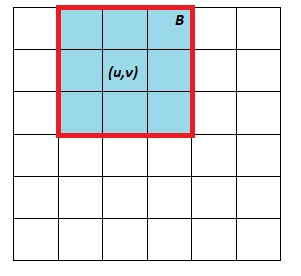
\includegraphics[width=0.3\textwidth]{fig/VentanaB.jpg}
	\caption{$B$ Neighborhood of size 3 $\times$ 3 centered in the pixel $(u,v)$ }
	\label{fig:Ventana B}
\end{figure}

\subsection{Division of the image into subregions}

The image $f$ is divided into subregions $W_1,W_2,\dots W_{x}$, so as to obtain local information from the image.
Let $B$ a window or structuring element, the domain $D$ corresponding to the window $B$ centered on $(u,v)$ is the set of subregions $W_{\{1,2,...,x\}}$,that touch some pixel of $B$.
%\begin{equation}
%\label{ventana}
%  \forall i, W_i \subseteq D_{(u,v)}\rightarrow \exists  \in D_{(u,v)}:x \in W_i
%\end{equation}   

In the figure \ref{fig:Sub-region} the image is divided into 4 subregions: $W_1$, $W_2$, $W_3$, $W_4$.  The region delimited by the window $B$ is shaded. As you can see, the domain
$D$ on which $w_l$ weights are calculated for $B$ will be the area corresponding to the $W_1$ sub-region .
 
%\begin{figure}
%	\centering
%		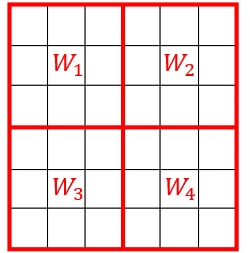
\includegraphics{fig/ventanas.png}
%	\caption{Imagen divida en 4 sub-regiones}
%	\label{fig:ventanas}
%\end{figure}


Note that the filter window does not have to to be of equalsized to sub-regions, as in this case. In the Figure \ref{fig:Sub-regiones} can be seen as the domain $D$ of which shall be calculated weights belong to the union of the sub-regions $W_1$ and $W_2$, as the window $B$ touches both. This is done to avoid that when comparing two identical colors may have different values, affected by the weights that come from two different subregions.  


\begin{figure}
	\centering
		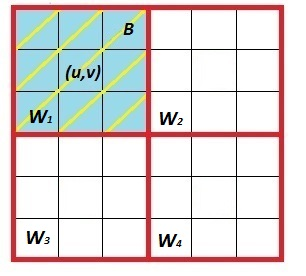
\includegraphics[width=0.3\textwidth]{fig/Sub-region.jpg}
	\caption{Domain when the window touches one subregion}
	\label{fig:Sub-region}
\end{figure}




\begin{figure}
	\centering
		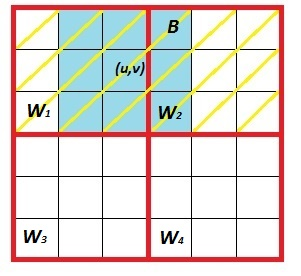
\includegraphics[width=0.3\textwidth]{fig/Sub-regiones.jpg}
	\caption{Domain when the window touches more than one subregion.}
	\label{fig:Sub-regiones}
\end{figure} In the case the user choose to have only one sub-region , that is not divide the image $f$, the weights will be calculated considering the whole picture $f$ as domain $D$.


In our tests, the input images of size $M \times N$ pixels, are divided into  $W_{\{1,2,...,x\}}$ subregions of $\left\lfloor\frac{M}{M'}\right\rfloor$ rows and $\left\lfloor\frac{N}{N'}\right\rfloor$ columns, where $\left\lfloor.\right\rfloor$ denotes the floor function. Thus, we have a new matrix of $M'$ rows y $N'$ columns, whose element is a subregion $W_l$.



\subsection{Application 1: Noise Removal}
Noise is a term used to refer to unwanted changes that may suffer a signal of any kind of nature during his capture, storage, transmission, processing or conversion \cite{tuzlukov2002signal}.

Noise in images is an undesirable product that adds misinformation. Noise occurs in digital images in the form of random variations in brightness or color information. 
Several mathematical models have been developed to simulate the generation of different types of existing noise. 

\subsubsection{Used noises} 

Given an input image $f$, the image $f'$ resulting from contaminating $f$ with some kind of noise and a vector $z = (z_1, z_2, z_3)$ in each element $z_l$  
corresponds to random variable; is defined the main noise models as follows:

\begin{itemize}
	
\item{Gaussian noise:}
It is an additive  statistical noise with a gaussian density function probability  \cite{davenport1958random}. Gaussian noise is expressed as follows:
\begin{equation}
\label{eq:gaussian_noise}
f'(x, y) = f(x, y) + z
\end{equation}
where each component $z_l$ is a random variable with normal distribution, $\mu$ average, $\sigma^2$ variance and it represents the value of noise added.

\item{Speckle noise:}
is a multiplicative noise with a uniform density function of probability, defined as follows: 

\begin{equation}
\label{eq:speckle}
f'(x, y) = f(x, y) + z \ast f(x, y)  
\end{equation}
where the operator $\ast$ symbolizes the Hadamard product or element by element. Each item $z_l$ is a random variable uniformly distributed with average $\mu$ and variance $\sigma^2$.

\item{Salt and pepper noise:}
this noise, unlike the Gaussian and Speckle noise, is not additive and multiplicative respect to the values of the original image. In the images affected with salt and pepper noise original values are replaced by bright values (salt) or dark values (pepper), that correspond to pulses inside to the signal. 

The salt pixels have the minimum possible value (zero)  and the pixel values pepper the maximum value possible ($2^k - 1$, where $k$ is the number of bits used to represent the intensity of each color component). The salt and pepper noise does not affect all pixels within an image, as with Gaussian and Speckle noises. The number of pixels in an image that are affected by salt and pepper noise parameter depends on the probability of noise $p$, which it is in the range $[0, 1]$.

The salt and pepper noise is modeled as follows:
\begin{equation}
\label{eq:salt_and_pepper}
f'(x, y)=\left\{ \begin{array}{cl}
s & \text{, with a probability } p/2 \\
r & \text{, with a probability } p/2 \\
f(x, y) & \text{, with a probability } 1 - p \\
\end{array}\right.
\end{equation}
where:\\ $s = (0, 0, 0)$ represents the salt noise,\\ $r = (2^k - 1, 2^k - 1, 2^k - 1 )$ represents the pepper noise.


\end{itemize}



In the Figure \ref{fig:ruido}(a) can see an image that is contaminated with Gaussian noise ( \ref{fig:ruido}(b)), speckle noise (\ref{fig:ruido}(c)), with salt and pepper noise (\ref{fig:ruido}(d)). 

%\begin{figure}[htbp]
%\centering
%\subfigure[Imagen original]{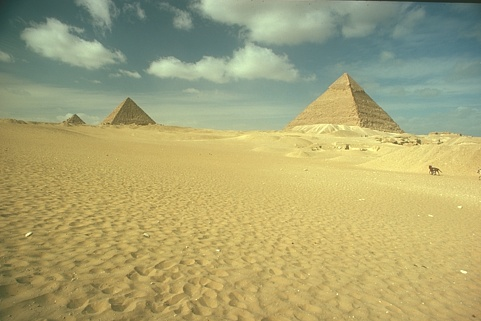
\includegraphics[width=73mm]{fig/Original_SinRuido.jpg}}
%\subfigure[Imagen con ruido gaussiano ($\sigma^2 = 0.05, \mu=0$)]{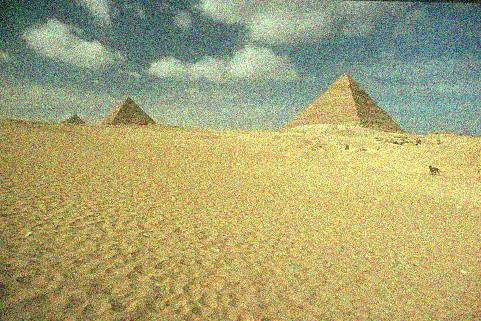
\includegraphics[width=73mm]{fig/img_gaussian_noise.jpg}}
%\subfigure[Imagen con ruido speckle ($\sigma^2 = 0.05, \mu=0$)]{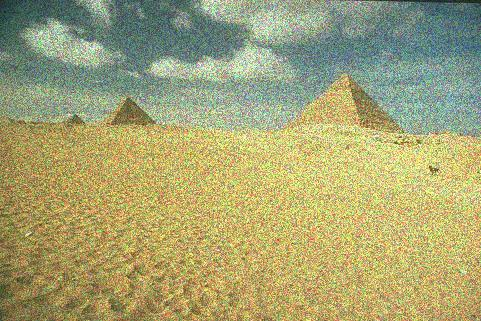
\includegraphics[width=73mm]{fig/img_speckle_noise.jpg}}
%\subfigure[Imagen con ruido sal y pimienta ($p = 0.05$)]{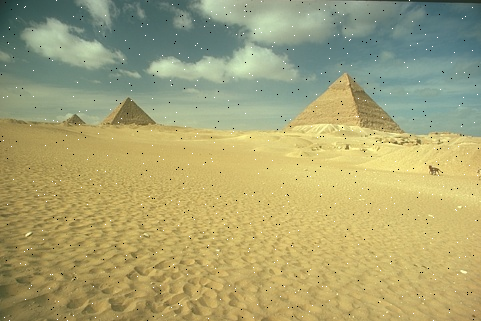
\includegraphics[width=73mm]{fig/img_salt_and_pepper_noise.jpg}}
%\caption{Imagen con diferentes tipos de ruidos.} \label{fig:ruido}
%\end{figure}


\begin{figure*}
	\makebox[\linewidth][c]{%
		\begin{subfigure}[b]{0.4\textwidth}
			\centering
			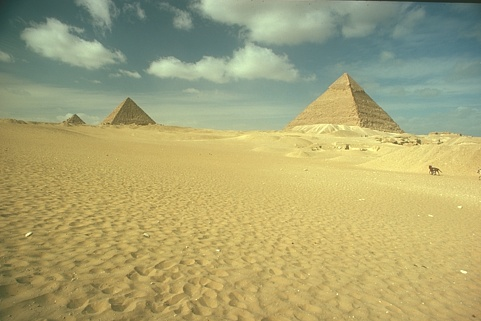
\includegraphics[width=0.95\textwidth]{fig/Original_SinRuido.jpg}
			\caption{Imagen original}
			\label{fig:original_sin_ruido}
		\end{subfigure}
		\begin{subfigure}[b]{0.4\textwidth}
			\centering
			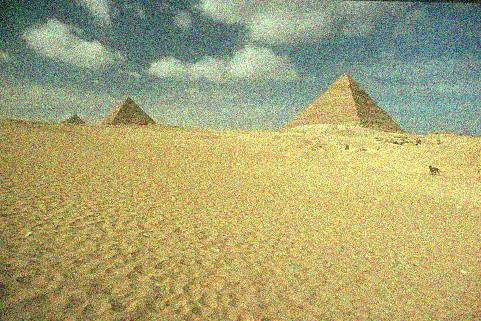
\includegraphics[width=0.95\textwidth]{fig/img_gaussian_noise.jpg}
			\caption{Image with gaussian noise ($\mu = 0; \sigma^2 = 0.05$)}
			\label{fig:con_ruido_gaussiano}
		\end{subfigure}
	}\\
	\makebox[\linewidth][c]{%
		\begin{subfigure}[b]{0.4\textwidth}
			\centering
			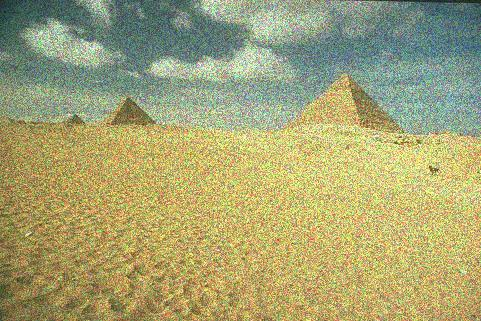
\includegraphics[width=0.95\textwidth]{fig/img_speckle_noise.jpg}
			\caption{Image with speckle noise ($\mu = 0; \sigma^2 = 0.05$)}
			\label{fig:con_ruido_speckle}
		\end{subfigure}
			\begin{subfigure}[b]{0.4\textwidth}
				\centering
				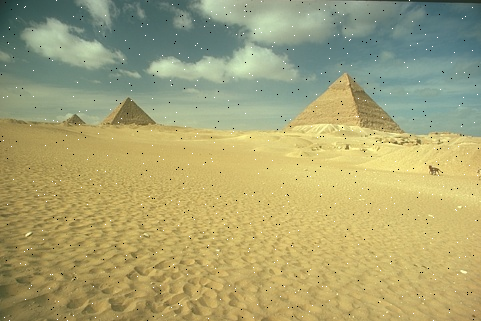
\includegraphics[width=0.95\textwidth]{fig/img_salt_and_pepper_noise.jpg}
				\caption{Image with salt and pepper noise ($p = 0.05$)}
				\label{fig:con_ruido_sal_y_pimienta}
			\end{subfigure}
	}\\
	\caption{Image with different kinds of noises.} \label{fig:ruido}
\end{figure*}





%Los par\'ametros utilizados en la generaci\'on de cada ruido fueron:

%\begin{itemize}
%	\item Ruido gaussiano: La media  $\mu=0$ y  la varianza $\sigma^2$ fue variando  entre los valores 0,01 y 0,17, haciendo pasos de 0,01. 
%	\item Ruido speckle: La media  $\mu=0$ y  la varianza $\sigma^2$ fue variando  entre los valores 0,01 y 0,17, haciendo pasos de 0,01. 
%	\item Ruido sal y pimienta: El valor de probabilidad $p$  de ocurrencia de un ruido sal o pimienta fue variando  entre los valores 0,01 y 0,17, haciendo pasos de 0,01. 
%\end{itemize}

%El valor de la varianza $\sigma^2$ para los ruidos gaussiano y speckle, as\'i como el valor de probabilidad $p$ de ocurriencia de un ruido sal o pimienta fue variando  de manera a observar como se comporta el filtro a medida que se va aumentando la cantidad de ruido.

So to evaluate the filter with the different types of ordering, is proposed to use a statistical metric used to measure how close they are forecasts or predictions of real results \cite{willmott2005advantages}.

Given an image $f$ and $g$ filtered image of $M \times N$ dimensions, the average absolute error of the filtered image is given by:
\begin{equation}
\label{MAE}
MAE(f,g) = \frac{1}{3\times M\times N}\sum_{j=1}^3 d_j
\end{equation} where: 


\begin{equation}
d_j = \sum_{\substack{u\in \{1, ..., M\}\\ v \in \{1, ..., N\}}} |[f(u,v)]_{j} - [g(u,v)]_{j}| 
\end{equation}

%\textsl{CDS (Color Distribution Similarity, Similaridad de Distribuciones de Color):} es una medida de similaridad para imágenes digitales a color basada en la diferencia de histogramas acumulados \cite{stricker1995similarity}.  La principal mejora de la diferencia de histogramas a color acumulado con respecto a la diferencia de histogramas a color radica; en que la diferencia de histograma a color acumulado obtiene todas las imágenes con similaridad perceptual a sus histogramas a color y de esta manera disminuye la probabilidad de obtener falsos negativos.

%Para determinar la similaridad de dos imágenes $f$ y $g$, con histogramas acumulados a color $\bar{H}^D_f$ y $\bar{H}^D_g$ en un dominio $D$, se calcula la diferencia entre $\bar{H}^D_f$ y $\bar{H}^D_g$: 
%\begin{equation}
%CDS(f,g) = \sqrt{\sum_{\substack{u\in \{1, ..., M\}\\ v \in \{1, ..., N\}}} (\bar{H}^D_f(f(u, v)) - \bar{H}^D_g(g(u, v)))^2}
%\end{equation}

%\include{anexos/graficos}
\subsubsection{Results}

Below are listed the codes used to abbreviate the names of the sorting methods that were the subject of experimentation:


\begin{itemize}
	\item ED: RGB Euclidean distance is used as a method of sorting colors \cite{ortiz2002procesamiento}.
	\item BM: RGB bit interleaving method is used as a ordering of colors \cite{chanussot1997bit}.
	\item LEX: RGB lexicographical ordering is used to sort the colors .
	\item ALEX: The RGB  $\alpha$ -lexicographic ordering is used 
	\cite{zamora2001comparative} for ordering colors.
	\item AMLEX: The RGB lexicographical $\alpha$-Module is used \cite{angulo2003morphological} for ordering colors.
	\item HLEX,  I→H→S lexicographical ordering is used to sort colors.
	\item DLAB, distance in L* a*b* is used as sorting method \cite{ortiz2002procesamiento}.
	\item MIN: the \ref{Transformacion} equation is used to add this transformation as the first component of the RGB lexicographical cascade , where:\\ 
$w = (Min(h_{f_1}^D), Min(h_{f_2}^D),Min(h_{f_3}^D))$.
	\item MAX: the \ref{Transformacion} equation is used to add this transformation as the first component of the RGB lexicographical cascade, where:\\ 
$w = (Max(h_{f_1}^D), Max(h_{f_2}^D),Max(h_{f_3}^D))$.
	\item MO1: the \ref{Transformacion} equation is used to add this transformation as the first component of the RGB lexicographical cascade, where:\\ 
$w = (minM_o(h_{f_1}^D), minM_o(h_{f_2}^D), minM_o(h_{f_3}^D))$.
	\item MO2: the \ref{Transformacion} equation is used to add this transformation as the first component of the RGB lexicographical cascade, where:\\ 
$w = (maxM_o(h_{f_1}^D), maxM_o(h_{f_2}^D), maxM_o(h_{f_3}^D))$.
	\item SMO: the \ref{Transformacion} equation is used to add this transformation as the first component of the RGB lexicographical cascade, where:\\ 
$w = (R(h_{f_1}^D), R(h_{f_2}^D), R(h_{f_3}^D))$.
	\item MEAN: the \ref{Transformacion} equation is used to add this transformation as the first component of the RGB lexicographical cascade, where:\\ 
$w = (Me(h_{f_1}^D), Me(h_{f_2}^D), Me(h_{f_3}^D))$.
	\item VAR: the \ref{Transformacion} equation is used to add this transformation as the first component of the RGB lexicographical cascade, where:\\ 
$w = (Var(h_{f_1}^D), Var(h_{f_2}^D), Var(h_{f_3}^D))$.
\end{itemize}

The filter used to eliminate different types of noise was the median. This filter consists to sort the colors within the filter window, and selecting the middle value to replace in the output image. So to avoid having a false color, the size of the filter window is usually odd ($3\times 3$ in our tests). The tests were made with 100 different images ( \cite{arbelaez2007berkeley} test images), polluted with noise: gaussiano, speckle, salt and pepper. In the case of Gaussian and Speckle noise, the parameter $\mu$ is set to $0$ and the $\sigma^2$ parameter was varied between $0.005$ and $0.165$, with $0.02$ increases. In the case of salt and pepper noise, the probability parameter $p$ was varied with the same values of the parameter $\sigma^2$ of Gaussian and  Speckle noise.

The Figure \ref{fig:imagen_ejemplo_ruido_gaussiano} corresponds to the original image of Figure \ref{fig:ruido} with $\sigma^2 = 0.105$ and $\mu = 0$. The result of applying the proposed order filters and other filters  evaluated on the contaminated image shown in the Figure \ref{fig:imagenes_resultado}.


\begin{figure}
	\centering
	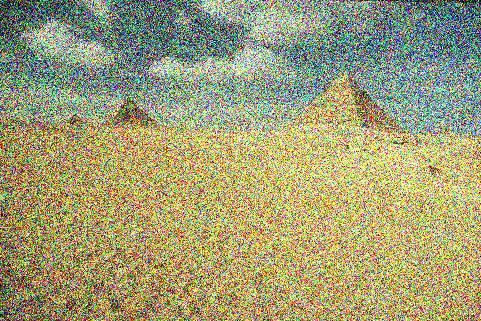
\includegraphics[width=0.38\textwidth]{fig/img_ruido_gaussian_83_0_105}
	\caption{Gaussian noise ($\mu = 0; \sigma^2 = 0.105$)}
	\label{fig:imagen_ejemplo_ruido_gaussiano}
\end{figure}


Should be noted that filtered images with the proposed order and with different weights are better visually to the state of the art, but they are perceptually very similar to each other, the difference between them is evident in the numerical results presented later in this section.

\begin{figure*}
	\makebox[\linewidth][c]{%
		\begin{subfigure}[b]{0.25\textwidth}
			\centering
			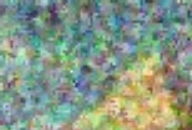
\includegraphics[width=0.95\linewidth]{fig/ALEX}
			\caption{ALEX}
			\label{fig:alex}
		\end{subfigure}
		\begin{subfigure}[b]{0.25\textwidth}
			\centering
			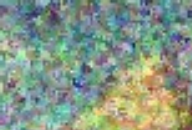
\includegraphics[width=0.95\linewidth]{fig/AMLEX}
			\caption{AMLEX}
			\label{fig:amlex}
		\end{subfigure}
		\begin{subfigure}[b]{0.25\textwidth}
			\centering
			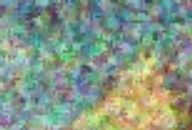
\includegraphics[width=0.95\linewidth]{fig/BM}
			\caption{BM}
			\label{fig:bm}
		\end{subfigure}
		\begin{subfigure}[b]{0.25\textwidth}
			\centering
			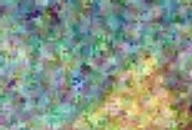
\includegraphics[width=0.95\linewidth]{fig/DLAB}
			\caption{DLAB}
			\label{fig:dlab}
		\end{subfigure}
	}\\
	\makebox[\linewidth][c]{%
		\begin{subfigure}[b]{0.25\textwidth}
			\centering
			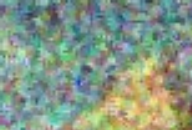
\includegraphics[width=0.95\linewidth]{fig/ED}
			\caption{ED}
			\label{fig:ed}
		\end{subfigure}
		\begin{subfigure}[b]{0.25\textwidth}
			\centering
			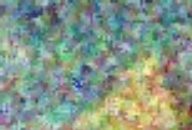
\includegraphics[width=0.95\linewidth]{fig/HLEX}
			\caption{HLEX}
			\label{fig:hlex}
			\phantomcaption
		\end{subfigure}
		\begin{subfigure}[b]{0.25\textwidth}
			\centering
			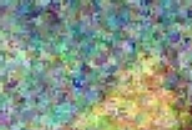
\includegraphics[width=0.95\linewidth]{fig/LEX}
			\caption{LEX}
			\label{fig:lex}
			\phantomcaption
		\end{subfigure}
		\begin{subfigure}[b]{0.25\textwidth}
			\centering
			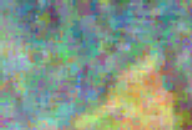
\includegraphics[width=0.95\linewidth]{fig/MAXM5}
			\caption{MAX}
			\label{fig:max}
			\phantomcaption
		\end{subfigure}
	}\\
	\makebox[\linewidth][c]{%
		\begin{subfigure}[b]{0.25\textwidth}
			\centering
			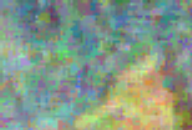
\includegraphics[width=0.95\linewidth]{fig/MEANM5}
			\caption{MEAN}
			\label{fig:mean}
			\phantomcaption
		\end{subfigure}
		\begin{subfigure}[b]{0.25\textwidth}
			\centering
			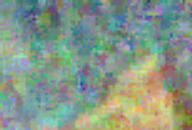
\includegraphics[width=0.95\linewidth]{fig/MINM5}
			\caption{MIN}
			\label{fig:min}
			\phantomcaption
		\end{subfigure}
		\begin{subfigure}[b]{0.25\textwidth}
			\centering
			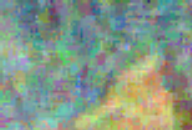
\includegraphics[width=0.95\linewidth]{fig/MOD2M5}
			\caption{MO2}
			\label{fig:mo2}
			\phantomcaption
		\end{subfigure}
		\begin{subfigure}[b]{0.25\textwidth}
			\centering
			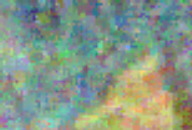
\includegraphics[width=0.95\linewidth]{fig/MODM5}
			\caption{MO1}
			\label{fig:mo1}
			\phantomcaption
		\end{subfigure}
	}\\
	\makebox[\linewidth][c]{%
		\begin{subfigure}[b]{0.25\textwidth}
			\centering
			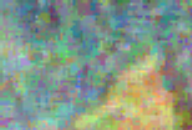
\includegraphics[width=0.95\linewidth]{fig/SMOM5}
			\caption{SMO}
			\label{fig:smo}
			\phantomcaption
		\end{subfigure}
		\begin{subfigure}[b]{0.25\textwidth}
			\centering
			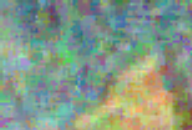
\includegraphics[width=0.95\linewidth]{fig/VARM5}
			\caption{VAR}
			\label{fig:var}
			\phantomcaption
		\end{subfigure}
	}\\
	\caption{Results of applying different filters evaluated on the image in Figure \ref{fig:imagen_ejemplo_ruido_gaussiano}. The image was divided into 5 x 5 subregions .}	
	\label{fig:imagenes_resultado}
\end{figure*}

For every noise and measuring a results table and graph trend curve of each filter with respect to the variation of noise parameter ($\sigma^2$ to Gaussian and speckle noise, and $p$ for salt and pepper noise). Each point represents the average of metric obtained by the filter to a noise parameter value $(\sigma^2\, MAE)$ or $(p,\,MAE)$. The corresponding curve of a filter is obtained by joining each pair of successive points of the filter with the line  (straight) passing through both points. This is done so as to be able to view the trend as a continuous function. The results tables order the filters as the total sum of all points on the graph curves. The filters shown in the top of the tables are those with the lowest values of the total sum of MAE obtained by each filter. In some cases, the state of the art filters perform better for less noise parameter values but are overcome by the filters proposed for higher noise parameter values. 

 The results of this section differ the order filters of each weight according to his domain settings. For reference, are added the suffix "WX" to the proposed filters codes, where X is a number representing the number of sub-regions in which the image was divided, with M'= $\sqrt{X}$ and N'= $\sqrt{X}$. When the neighborhood (marked by the filter window) is the domain, suffix "B" is used.

%Para poder seleccionar varias columnas de una vez
\pgfplotstableset{
	my multistyler/.style 2 args={
		@my multistyler/.style={display columns/##1/.append style={#2}},
		@my multistyler/.list={#1}
	}
}

\pgfplotstableread[
col sep = tab,
header=has colnames,
]
{anexos/files/color_and_marker_by_filter.txt}{\colorbyfilter}



%mae gaussiano
\pgfplotstableread[
col sep = tab,
header=has colnames,
comment chars={P},
]
{anexos/files/ventanas_mae_gaussian.txt}{\ventanasmaegaussian}
\pgfplotstablegetcolsof{\ventanasmaegaussian}
\pgfmathsetmacro{\C}{\pgfplotsretval - 1}
\pgfmathsetmacro{\B}{\C-1}
\pgfplotstablegetrowsof{\ventanasmaegaussian}
\pgfmathsetmacro{\R}{\pgfplotsretval - 1}
\pgfmathsetmacro{\F}{6} %cantidad de filas a mostrar en las tablas de resumen

\pgfplotstabletranspose[
colnames from=p,
input colnames to=p
]\ventanasmaegaussiannew{anexos/files/ventanas_mae_gaussian.txt}


\begin{table}[!h]
	\centering
	\caption{Ruido gaussiano. Sumatoria de MAE por $\sigma^2$}
	\pgfkeys{/pgf/number format/precision=4}
	\pgfplotstabletypeset[
	col sep=tab,
	%header=has colnames,
	columns = {[index]0, [index]10},
	columns/P/.style = {column name = Suma},
	columns/p/.style = {column name = Filtro},
	%skip rows between index={6}{25},
	every first column/.style={
		string type,
		column type/.add={|}{|},
	},
	every head row/.style={
		before row=\hline,
		after row=\hline
	},
	every last column/.style={column type/.add={}{|}},
	every last row/.style={
		after row=\hline,
	},
	]{\ventanasmaegaussiannew}
	\label{tabla:gaussian_mae}
\end{table}

%mae sal y pimienta
\pgfplotstableread[
col sep = tab,
header=has colnames,
comment chars={P},
]
{anexos/files/ventanas_mae_salt_and_pepper.txt}{\ventanasmaesaltandpepper}

\pgfplotstabletranspose[
colnames from=p,
input colnames to=p
]\ventanasmaesaltandpeppernew{anexos/files/ventanas_mae_salt_and_pepper.txt}


\begin{table}[htbp]
	\centering
	\caption{Salt and pepper noise. Summation of MAE by $p$}
	\pgfkeys{/pgf/number format/precision=4}
	\pgfplotstabletypeset[
	col sep=tab,
	%header=has colnames,
	columns = {[index]0, [index]10},
	columns/P/.style = {column name = Suma},
	columns/p/.style = {column name = Filtro},
	%skip rows between index={6}{25},
	every first column/.style={
		string type,
		column type/.add={|}{|},
	},
	every head row/.style={
		before row=\hline,
		after row=\hline
	},
	every last column/.style={column type/.add={}{|}},
	every last row/.style={
		after row=\hline,
	},
	]{\ventanasmaesaltandpeppernew}
	\label{tabla:salt_and_pepper_mae}
\end{table}

%mae speckle
\pgfplotstableread[
col sep = tab,
header=has colnames,
comment chars={P},
]
{anexos/files/ventanas_mae_speckle.txt}{\ventanasmaespeckle}

\pgfplotstabletranspose[
colnames from=p,
input colnames to=p
]\ventanasmaespecklennew{anexos/files/ventanas_mae_speckle.txt}


\begin{table}[htbp]
	\centering
	\caption{Ruido speckle. Sumatoria de MAE por $\sigma^2$}
	\pgfkeys{/pgf/number format/precision=4}
	\pgfplotstabletypeset[
	col sep=tab,
	%header=has colnames,
	columns = {[index]0, [index]10},
	columns/P/.style = {column name = Suma},
	columns/p/.style = {column name = Filtro},
	%skip rows between index={6}{25},
	every first column/.style={
		string type,
		column type/.add={|}{|},
	},
	every head row/.style={
		before row=\hline,
		after row=\hline
	},
	every last column/.style={column type/.add={}{|}},
	every last row/.style={
		after row=\hline,
	},
	]{\ventanasmaegaussiannew}
	\label{tabla:speckle_mae}
\end{table}


\begin{figure*}[htbp]
	\centering
	\begin{tikzpicture}[spy using outlines={circle, magnification=9.5, size=3.5cm, connect spies}]
	\begin{axis}[
	xmax = 0.175,
	legend style={mark options={scale=1.5}},
	xlabel={$\sigma^2$},
	ylabel={MAE},
	legend pos=outer north east,
	height=0.5\textwidth,
	width=0.6\textwidth,
	tick label style={/pgf/number format/fixed,
		/pgf/number format/precision=4}
	]
	\foreach \n in {\C,\B,...,1} {
		\pgfplotstablegetcolumnnamebyindex{\n}\of{\ventanasmaegaussian}\to{\colname}
		\pgfplotstablegetelem{0}{\colname}\of{\colorbyfilter}
		\let\color=\pgfplotsretval
		\pgfplotstablegetelem{1}{\colname}\of{\colorbyfilter}
		\let\marca=\pgfplotsretval
		\edef\temp{
			\noexpand\addplot+[\color, mark=\marca, solid, mark options={mark size = 1.5, fill=\color!70}] 
		}
		\temp	
		table[x=p, y index=\n]{\ventanasmaegaussian};
		
		\addlegendentryexpanded{\colname}
	}%
	\pgfplotstablegetelem{\R}{[index]1}\of{\ventanasmaegaussian}
	\let\ytozoom=\pgfplotsretval
	\coordinate (spypoint) at (axis cs:0.165,\ytozoom);
	\coordinate (spyviewer) at (axis cs:0.12,17);
	\spy on (spypoint) in node [fill=white] at (spyviewer);
	\end{axis}
	\end{tikzpicture}
	\caption{Ruido gaussiano. MAE por $\sigma^2$}
	\label{fig:gaussian_mae}
\end{figure*}

\begin{figure*}[htbp]
	\centering
	\begin{tikzpicture}[spy using outlines={circle, magnification=9.5, size=3.5cm, connect spies}]
	\begin{axis}[
	xmax = 0.175,
	legend style={mark options={scale=1.5}},
	xlabel={$p$},
	ylabel={MAE},
	legend pos=outer north east,
	height=0.5\textwidth,
	width=0.6\textwidth,
	tick label style={/pgf/number format/fixed,
		/pgf/number format/precision=4}
	]
	\foreach \n in {\C,\B,...,1} {
		\pgfplotstablegetcolumnnamebyindex{\n}\of{\ventanasmaesaltandpepper}\to{\colname}
		\pgfplotstablegetelem{0}{\colname}\of{\colorbyfilter}
		\let\color=\pgfplotsretval
		\pgfplotstablegetelem{1}{\colname}\of{\colorbyfilter}
		\let\marca=\pgfplotsretval
		\edef\temp{
			\noexpand\addplot+[\color, mark=\marca, solid, mark options={mark size = 1.5, fill=\color!70}] 
		}
		\temp	
		table[x=p, y index=\n]{\ventanasmaesaltandpepper};
		
		\addlegendentryexpanded{\colname}	
	}%
	\pgfplotstablegetelem{\R}{[index]1}\of{\ventanasmaesaltandpepper}
	\let\ytozoom=\pgfplotsretval
	\coordinate (spypoint) at (axis cs:0.165,\ytozoom);
	\coordinate (spyviewer) at (axis cs:0.04,6.15);
	\spy on (spypoint) in node [fill=white] at (spyviewer);
	\end{axis}
	\end{tikzpicture}
	\caption{Salt and pepper noise. MAE by $p$}
	\label{fig:salt_and_pepper_mae}
\end{figure*}


\begin{figure*}[htbp]
	\centering
	\begin{tikzpicture}[spy using outlines={circle, magnification=9.5, size=3.5cm, connect spies}]
	\begin{axis}[
	xmax = 0.175,
	legend style={mark options={scale=1.5}},
	xlabel={$p$},
	ylabel={MAE},
	legend pos=outer north east,
	height=0.5\textwidth,
	width=0.6\textwidth,
	tick label style={/pgf/number format/fixed,
		/pgf/number format/precision=4}
	]
	\foreach \n in {\C,\B,...,1} {
		\pgfplotstablegetcolumnnamebyindex{\n}\of{\ventanasmaespeckle}\to{\colname}
		\pgfplotstablegetelem{0}{\colname}\of{\colorbyfilter}
		\let\color=\pgfplotsretval
		\pgfplotstablegetelem{1}{\colname}\of{\colorbyfilter}
		\let\marca=\pgfplotsretval
		\edef\temp{
			\noexpand\addplot+[\color, mark=\marca, solid, mark options={mark size = 1.5, fill=\color!70}] 
		}
		\temp	
		table[x=p, y index=\n]{\ventanasmaespeckle};
		
		\addlegendentryexpanded{\colname}	
	}%
	\pgfplotstablegetelem{\R}{[index] 1}\of{\ventanasmaespeckle}
	\let\ytozoom=\pgfplotsretval
	\coordinate (spypoint) at (axis cs:0.165,\ytozoom);
	\coordinate (spyviewer) at (axis cs:0.12,13);
	\spy on (spypoint) in node [fill=white] at (spyviewer);
	\end{axis}
	\end{tikzpicture}
	\caption{Speckle noise. MAE by $\sigma^2$}
	\label{fig:speckle_mae}
\end{figure*}

%
%%cds gaussiano
%\pgfplotstableread[
%col sep = tab,
%header=has colnames,
%comment chars={P},
%]
%{anexos/files/ventanas_cds_gaussian.txt}{\ventanascdsgaussian}
%\pgfplotstablegetcolsof{\ventanascdsgaussian}
%\pgfmathsetmacro{\C}{\pgfplotsretval-1}
%
%
%\begin{figure*}
%	\centering
%	\begin{tikzpicture}[spy using outlines={circle, magnification=9.5, size=3.5cm, connect spies}]
%	\begin{axis}[
%	xmax = 0.175,
%	legend style={mark options={scale=1.5}},
%	xlabel={$\sigma^2$},
%	ylabel={CDS},
%	legend pos=outer north east,
%	height=0.5\textwidth,
%	width=0.6\textwidth,
%	tick label style={/pgf/number format/fixed,
%		/pgf/number format/precision=4}
%	]
%	\foreach \n in {\C,\B,...,1} {
%		\pgfplotstablegetcolumnnamebyindex{\n}\of{\ventanascdsgaussian}\to{\colname}
%		\pgfplotstablegetelem{0}{\colname}\of{\colorbyfilter}
%		\let\color=\pgfplotsretval
%		\pgfplotstablegetelem{1}{\colname}\of{\colorbyfilter}
%		\let\marca=\pgfplotsretval
%		\edef\temp{
%			\noexpand\addplot+[\color, mark=\marca, solid, mark options={mark size = 1.5, fill=\color!70}] 
%		}
%		\temp	
%		table[x=p, y index=\n]{\ventanascdsgaussian};
%		
%		\addlegendentryexpanded{\colname}
%	}%
%	\pgfplotstablegetelem{\R}{[index]1}\of{\ventanascdsgaussian}
%	\let\ytozoom=\pgfplotsretval
%	\coordinate (spypoint) at (axis cs:0.165,\ytozoom);
%	\coordinate (spyviewer) at (axis cs:0.1,22000000);
%	\spy on (spypoint) in node [fill=white] at (spyviewer);
%	\end{axis}
%	\end{tikzpicture}
%	\caption{Ruido gaussiano. CDS por $\sigma^2$}
%	\label{fig:gaussian_cds}
%\end{figure*}
%
%
%\begin{table*}
%	\small
%	\centering
%	\caption{Ruido gaussiano. $CDS \times 10^7$ por $\sigma^2$}
%	\pgfkeys{/pgf/number format/precision=5}
%	\pgfplotstabletypeset[
%	col sep=tab,
%	header=has colnames,
%	every first column/.style={
%		string type,
%		column type/.add={|}{|}
%	},
%	every head row/.style={
%		before row=\hline,
%		after row=\hline
%	},
%	every last column/.style={column type/.add={}{|}},
%	every last row/.style={
%		after row=\hline,
%	},
%	every row 0 column 1/.style={
%		postproc cell content/.style={
%			@cell content/.add={$\bf}{$}
%		}
%	},
%	every row 0 column 2/.style={
%		postproc cell content/.style={
%			@cell content/.add={$\bf}{$}
%		}
%	},
%	every row 0 column 3/.style={
%		postproc cell content/.style={
%			@cell content/.add={$\bf}{$}
%		}
%	},
%	every row 0 column 4/.style={
%		postproc cell content/.style={
%			@cell content/.add={$\bf}{$}
%		}
%	},
%	every row 0 column 5/.style={
%		postproc cell content/.style={
%			@cell content/.add={$\bf}{$}
%		}
%	},
%	every row 0 column 6/.style={
%		postproc cell content/.style={
%			@cell content/.add={$\bf}{$}
%		}
%	},
%	every row 1 column 7/.style={
%		postproc cell content/.style={
%			@cell content/.add={$\bf}{$}
%		}
%	},
%	every row 1 column 8/.style={
%		postproc cell content/.style={
%			@cell content/.add={$\bf}{$}
%		}
%	},
%	every row 1 column 9/.style={
%		postproc cell content/.style={
%			@cell content/.add={$\bf}{$}
%		}
%	},
%	my multistyler={1,...,17}{
%		divide by={10000000}
%	},
%	]{anexos/files/ventanas_cds_gaussian_tabla.txt}
%	\label{tabla:gaussian_cds}
%\end{table*}
%
%%cds sal y pimienta
%\pgfplotstableread[
%col sep = tab,
%header=has colnames,
%comment chars={P},
%]
%{anexos/files/ventanas_cds_salt_and_pepper.txt}{\ventanascdssaltandpepper}
%
%
%\begin{figure*}
%	\centering
%	\begin{tikzpicture}[spy using outlines={circle, magnification=9.5, size=3.5cm, connect spies}]
%	\begin{axis}[
%	xmax = 0.175,
%	legend style={mark options={scale=1.5}},
%	xlabel={$p$},
%	ylabel={CDS},
%	legend pos=outer north east,
%	height=0.5\textwidth,
%	width=0.6\textwidth,
%	tick label style={/pgf/number format/fixed,
%		/pgf/number format/precision=4}
%	]
%	\foreach \n in {\C,\B,...,1} {
%		\pgfplotstablegetcolumnnamebyindex{\n}\of{\ventanascdssaltandpepper}\to{\colname}
%		\pgfplotstablegetelem{0}{\colname}\of{\colorbyfilter}
%		\let\color=\pgfplotsretval
%		\pgfplotstablegetelem{1}{\colname}\of{\colorbyfilter}
%		\let\marca=\pgfplotsretval
%		\edef\temp{
%			\noexpand\addplot+[\color, mark=\marca, solid, mark options={mark size = 1.5, fill=\color!70}] 
%		}
%		\temp	
%		table[x=p, y index=\n]{\ventanascdssaltandpepper};
%		
%		\addlegendentryexpanded{\colname}
%	}%
%	\pgfplotstablegetelem{\R}{MINW9}\of{\ventanascdssaltandpepper}
%	\let\ytozoom=\pgfplotsretval
%	\coordinate (spypoint) at (axis cs:0.165,\ytozoom);
%	\coordinate (spyviewer) at (axis cs:0.137,10170000);
%	\spy on (spypoint) in node [fill=white] at (spyviewer);
%	\end{axis}
%	\end{tikzpicture}
%	\caption{Ruido sal y pimienta. CDS por $p$}
%	\label{fig:salt_and_pepper_cds}
%\end{figure*}
%
%
%\begin{table*}
%	\centering
%	\small
%	\caption{Ruido sal y pimienta. $CDS \times 10^7$ por $p$}
%	\pgfkeys{/pgf/number format/precision=4}
%	\pgfplotstabletypeset[
%	col sep=tab,
%	header=has colnames,
%	every first column/.style={
%		string type,
%		column type/.add={|}{|},
%	},
%	every head row/.style={
%		before row=\hline,
%		after row=\hline
%	},
%	every last column/.style={column type/.add={}{|}},
%	every last row/.style={
%		after row=\hline,
%	},
%	every row 0 column 1/.style={
%		postproc cell content/.style={
%			@cell content/.add={$\bf}{$}
%		}
%	},
%	every row 0 column 2/.style={
%		postproc cell content/.style={
%			@cell content/.add={$\bf}{$}
%		}
%	},
%	every row 0 column 3/.style={
%		postproc cell content/.style={
%			@cell content/.add={$\bf}{$}
%		}
%	},
%	every row 0 column 4/.style={
%		postproc cell content/.style={
%			@cell content/.add={$\bf}{$}
%		}
%	},
%	every row 0 column 5/.style={
%		postproc cell content/.style={
%			@cell content/.add={$\bf}{$}
%		}
%	},
%	every row 0 column 6/.style={
%		postproc cell content/.style={
%			@cell content/.add={$\bf}{$}
%		}
%	},
%	every row 0 column 7/.style={
%		postproc cell content/.style={
%			@cell content/.add={$\bf}{$}
%		}
%	},
%	every row 0 column 8/.style={
%		postproc cell content/.style={
%			@cell content/.add={$\bf}{$}
%		}
%	},
%	every row 0 column 9/.style={
%		postproc cell content/.style={
%			@cell content/.add={$\bf}{$}
%		}
%	},
%	my multistyler={1,...,17}{
%		divide by={10000000}
%	},
%	]{anexos/files/ventanas_cds_salt_and_pepper_tabla.txt}
%	\label{tabla:salt_and_pepper_cds}
%\end{table*}
%
%%cds speckle
%\pgfplotstableread[
%col sep = tab,
%header=has colnames,
%comment chars={P},
%]
%{anexos/files/ventanas_cds_speckle.txt}{\ventanascdspeckle}
%
%
%\begin{figure*}
%	\centering
%	\begin{tikzpicture}[spy using outlines={circle, magnification=9.5, size=3.5cm, connect spies}]
%	\begin{axis}[
%	xmax = 0.175,
%	legend style={mark options={scale=1.5}},
%	xlabel={$\sigma^2$},
%	ylabel={CDS},
%	legend pos=outer north east,
%	height=0.5\textwidth,
%	width=0.6\textwidth,
%	tick label style={/pgf/number format/fixed,
%		/pgf/number format/precision=4}
%	]
%	\foreach \n in {\C,\B,...,1} {
%		\pgfplotstablegetcolumnnamebyindex{\n}\of{\ventanascdspeckle}\to{\colname}
%		\pgfplotstablegetelem{0}{\colname}\of{\colorbyfilter}
%		\let\color=\pgfplotsretval
%		\pgfplotstablegetelem{1}{\colname}\of{\colorbyfilter}
%		\let\marca=\pgfplotsretval
%		\edef\temp{
%			\noexpand\addplot+[\color, mark=\marca, solid, mark options={mark size = 1.5, fill=\color!70}] 
%		}
%		\temp	
%		table[x=p, y index=\n]{\ventanascdspeckle};
%		
%		\addlegendentryexpanded{\colname}
%	}%
%	\pgfplotstablegetelem{\R}{SMOW9}\of{\ventanascdspeckle}
%	\let\ytozoom=\pgfplotsretval
%	\coordinate (spypoint) at (axis cs:0.165,\ytozoom);
%	\coordinate (spyviewer) at (axis cs:0.12,20000000);
%	\spy on (spypoint) in node [fill=white] at (spyviewer);
%	\end{axis}
%	\end{tikzpicture}
%	\caption{Ruido speckle. CDS por $\sigma^2$}
%	\label{fig:speckle_cds}
%\end{figure*}
%
%
%\begin{table*}
%	\centering
%	\small
%	\caption{Ruido speckle. $CDS \times 10^7$ por $\sigma^2$}
%	\pgfkeys{/pgf/number format/precision=5}
%	\pgfplotstabletypeset[
%	col sep=tab,
%	header=has colnames,
%	every first column/.style={
%		string type,
%		column type/.add={|}{|},
%	},
%	every head row/.style={
%		before row=\hline,
%		after row=\hline
%	},
%	every last column/.style={column type/.add={}{|}},
%	every last row/.style={
%		after row=\hline,
%	},
%	every row 0 column 1/.style={
%		postproc cell content/.style={
%			@cell content/.add={$\bf}{$}
%		}
%	},
%	every row 0 column 2/.style={
%		postproc cell content/.style={
%			@cell content/.add={$\bf}{$}
%		}
%	},
%	every row 0 column 3/.style={
%		postproc cell content/.style={
%			@cell content/.add={$\bf}{$}
%		}
%	},
%	every row 0 column 4/.style={
%		postproc cell content/.style={
%			@cell content/.add={$\bf}{$}
%		}
%	},
%	every row 0 column 5/.style={
%		postproc cell content/.style={
%			@cell content/.add={$\bf}{$}
%		}
%	},
%	every row 0 column 6/.style={
%		postproc cell content/.style={
%			@cell content/.add={$\bf}{$}
%		}
%	},
%	every row 0 column 7/.style={
%		postproc cell content/.style={
%			@cell content/.add={$\bf}{$}
%		}
%	},
%	every row 0 column 8/.style={
%		postproc cell content/.style={
%			@cell content/.add={$\bf}{$}
%		}
%	},
%	every row 0 column 9/.style={
%		postproc cell content/.style={
%			@cell content/.add={$\bf}{$}
%		}
%	},
%	my multistyler={1,...,17}{
%		divide by={10000000}
%	},
%	]{anexos/files/ventanas_cds_speckle_tabla.txt}
%	\label{tabla:speckle_cds}
%\end{table*}
\normalsize

In the Figure \ref{fig:gaussian_mae} the trend curves of the filters applied to images contaminated with gaussian noise are observed . As can be seen, for gaussian noise, the best filter was the proposed using SMO, MAX, VAR and MEAN for calculating weight vector. Table \ref{tabla:gaussian_mae}  contains the total sum of the points on the trend curve  by sorting method.

Figure \ref{fig:salt_and_pepper_mae} shows the trend curves of the filters applied to images contaminated with salt and pepper noise. In this case the filter to obtained the lowest overall average and whose curve is placed below all others was ED. The MAX, SMO, VAR and MEAN filters showed better performances after ED. Table \ref{tabla:salt_and_pepper_mae} contains the total sum of the points on the curve trend by sorting method.

In the Figure \ref{fig:speckle_mae} there are the trend curves of the filters applied to images contaminated with speckle noise .The SMO, MAX and VAR filters obtained the best results. The filter SW9 obtained the best results for all points of the curve. The ED filter resulted the best of the state of the art. Table \ref{tabla:speckle_mae} contains the total sum of the points in the trend curve by sorting method in ascending sort.

%Desde la Figura \ref{fig:gaussian_cds} en adelante se ilustran los resultados para la métrica CDS. La Figura \ref{fig:gaussian_cds} muestra los resultados para el ruido gaussiano en la mencionada métrica. Los mejores filtros resultaron ser nuevamente los propuestos (SMO, MAX, VAR, MEAN) excepto MO1, MO2 y MIN que fueron superados por el mejor filtro del estado del arte, ED. En el zoom se hace visible la diferencia entre los filtros propuestos y el filtro ED. El Cuadro \ref{tabla:gaussian_cds} proporciona los valores numéricos a partir de los cuales se formaron las gráficas mencionadas; en el mismo puede observarse que el filtro SMOW9 obtuvo los mejores resultados hasta el punto $0.105$, desde el punto $0.125$ en adelante MAXW9 obtuvo los mejores resultados.
%
%La Figura \ref{fig:salt_and_pepper_cds} proporciona los resultados de la métrica CDS para el ruido sal y pimienta. Nuevamente, tal y como ocurrió con la métrica MAE, los filtros propuestos no resultaron tan eficaces para este ruido. En la figura se puede ver la marcada ventaja que el filtro DLAB posee por sobre los demás. El Cuadro \ref{tabla:gaussian_cds} brinda los valores numéricos utilizados en la construcción de las curvas mencionadas. Cabe resaltar que para la métrica MAE el ordenamiento ED fue el mejor filtro, no así  en la métrica CDS, que resultó ser el filtro con ordenameinto DLAB.  
%
%Por último, la Figura \ref{fig:speckle_cds} posee los valores de la métrica CDS para filtros aplicados sobre imágenes contaminadas con el ruido speckle. El Cuadro \ref{tabla:speckle_cds} posee los resultados numéricos de dichos gráficos de curvas. En este caso se puede observar nuevamente un solapamiento de las curvas correspondientes a los filtros propuestos (MAX, SMO, VAR, MEAN), pero a una distancia evidente de las curvas correspondientes al estado del arte, de entre las cuales el mejor fue ED. El filtro SMOW9 obtuvo los mejores resultados en todos los puntos de $\sigma^2$.

The following two applications use morphological mathematical. Operators are not purely morphological, since it can not guarantee its theoretical properties, as idempotency for opening and closing. In the Figure \ref{fig:ContraEjemplo} you can see a counter-example, where the opening operator is not  idempotent ($f\circ B \neq (f\circ B) \circ B$). To the synthetic image of the Figure \ref{fig:ContraEjemplo}(a) is applied an opening with 3 x 3 structural element, where the domain $D$ of the image is the neighborhood of the structuring element itself, and the function applied to each color component is the average inside $D$, resulting image of the Figure \ref{fig:ContraEjemplo}(b). To image of the Figure  \ref{fig:ContraEjemplo}(b) is applied again the operator of opening with the same structuring element and where the domain $D$ is also the neighborhood of the structuring element itself, resulting the image of the Figure \ref{fig:ContraEjemplo}(c). The resulting image is not equal to the previous one, this can be visualized on the image \ref{fig:ContraEjemplo}(c), which is the result of performing the difference between the two images. Thus it is demonstrated that the opening operator is not idempotent , the same occurs for the closing operator.


\begin{figure*}
	\makebox[\linewidth][c]{%
		\begin{subfigure}[b]{0.25\textwidth}
			\centering
			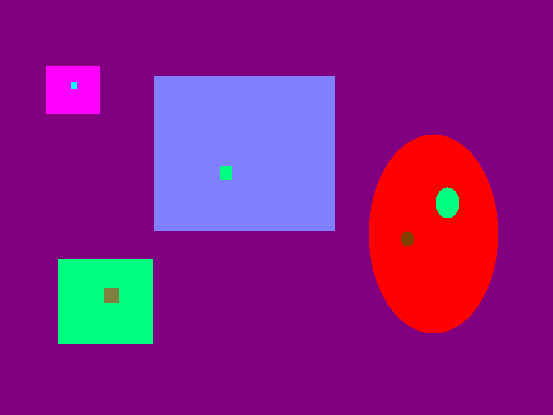
\includegraphics[width=0.95\linewidth]{fig/ImgCortes.png}
			\caption{Synthetic image}
			\label{fig:ImaSin}
		\end{subfigure}
		\begin{subfigure}[b]{0.25\textwidth}
			\centering
			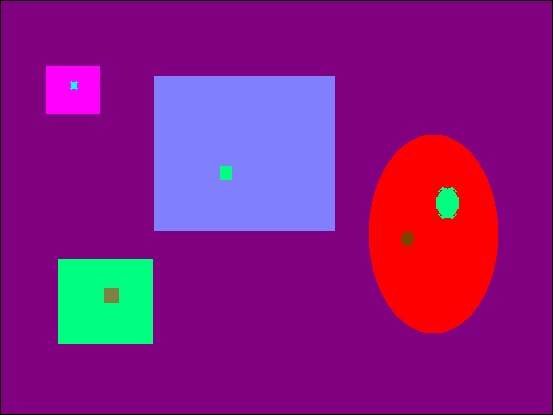
\includegraphics[width=0.95\linewidth]{fig/Apertura1.png}
			\caption{Aperture of the image (a)}
			\label{fig:Apert1}
		\end{subfigure}
		\begin{subfigure}[b]{0.25\textwidth}
			\centering
			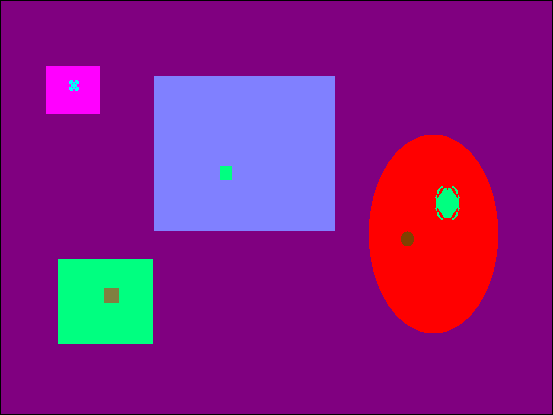
\includegraphics[width=0.95\linewidth]{fig/Apertura2.png}
			\caption{Aperture of the image (b)}
			\label{fig:Apert2}
		\end{subfigure}
		\begin{subfigure}[b]{0.25\textwidth}
			\centering
			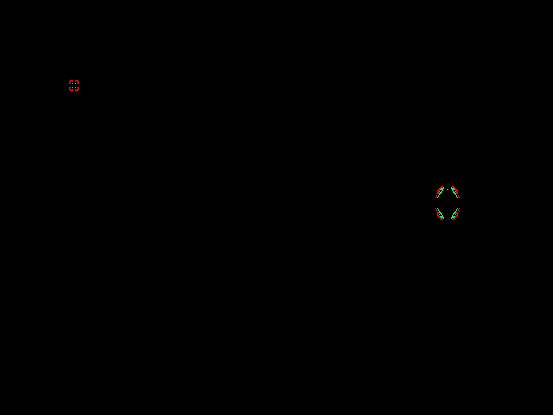
\includegraphics[width=0.95\linewidth]{fig/DiferenciaApertura.png}
			\caption{Difference between (b) and (c)}
			\label{fig:Apert1}
		\end{subfigure}
	}\\
	\caption{A counter-example shows that openness is not idempotent with the ordering proposed.}	
	\label{fig:ContraEjemplo}
\end{figure*}

This is because a color can be more or less than other color in a domain $D$, but not in another domain, because the extracted information in the form of weights (result of applying a function) may be different. Even in the same domain but in the next iteration (product of reapplying the same operator) they can vary the weights, since the extracted information also varies from one iteration to another. In the literature these operators are called pseudo-operators \cite{hanbury2001morphological,aptoula2007pseudo,aptoula2008alpha,angulo2010pseudo,chen2002pseudo}. 

Top-hat transform is widely used in different applications \cite{soille2013morphological,mukhopadhyay2000multiscale,soille1997note,bai2010analysis,bai2010infrared,bai2010analysis1}. As we mentioned earlier white top-hat transform extracts the bright  regions of the image and  top-hat transform the dark areas of the image.

\subsection{Application 2: Contrast improving}
 A basic idea of improving contrast of image $f$ is to add the bright regions of the image $f$  and subtract the dark regions of the image $f$  as follows \cite{soille2013morphological}:
\begin{equation}
\label{contraste}
Contrast(f) = f + WTH(f) - BTH(f) 
\end{equation}


The effectiveness of the application of contrast improvement it is determined using the method called Color Enhancement Factor (CEF) which quantifies the level of contrast enhancement of an image as mentioned in \cite{susstrunk2003color}. This method applied to the image $f$ is based on the average and standard deviation of two axes of a simple contrary color representation with $\gamma = f_1 - f_2$ y $\beta = \frac{1}{2}(f_1 + f_2) - f_3$.
The equation \ref{eq:cef} represents the level of contrast enhancement of the image $f$ as follows:

\begin{equation}
CM(f)=\sqrt{\sigma_{\gamma}^{2} + \sigma_{\beta}^{2}} + \sqrt{\mu_{\gamma}^{2} + \mu_{\beta}^{2}}
\label{eq:cef}
\end{equation} Where $\sigma_{\gamma}$ and $\sigma_{\beta}$ correspond to the standard deviation of $\gamma$ and $\beta$ respectively. Similarly, $\mu_{\gamma}$ and $\mu_{\beta}$ corresponds to the respectively mean.

Then, the CEF is calculated by the ratio of the $f'$ image and $f$ original image:

\begin{equation}
CEF = \frac{CM(f^{'})}{CM(f)}
\label{cef}
\end{equation}

Where $CM(f^{'})$ is the value obtained from the contrasted image $f'$ product of applying the equation \ref{eq:cef} and $CM(f)$ represents the result of applying the equation \ref{eq:cef} to the original image $f$. If the result is $> 1$ then the metric of the equation \ref{cef} indicates an improvement in the contrast, otherwise, metric indicates no contrast enhancement.



\subsubsection{Results}
The tests were made with 100 test images of \cite{arbelaez2007berkeley} and were used the same abbreviations as in the previous experiment to differentiate the sorting methods with different domain decomposition. 
In the \ref{tab:EXP_N1}  can see the results of the various iterations (iter) of contrast enhancement algorithm (applied several times the equation \ref{contraste} to the same image).  
Is observed that SMOB has better results in all the iterations, followed by the variance VARB and then follow the other methods. The improvement using SMOB as it grows the amount  of iterations is approximately 3\% and the difference with the second and third is of 0.30\% and 2.25\% on average in each of the iterations.
It can be seen that as the number of iterations increases also improves the contrast according to the mentioned metric , being also important the domain and sorting method used.

\begin{table}
\caption{Contrast improvement}
\label{tab:EXP_N1}
\begin{tabular}{ccccccccc}
\hline METODO& iter1&iter2&iter3&iter4\\
\hline  \textbf{SMOB}& \textbf{1,03482}& \textbf{1,03482}& \textbf{1,06084}& \textbf{1,08889}\\
\hline  \textbf{VARB}& \textbf{1,0329}& \textbf{1,0329}& \textbf{1,05798}& \textbf{1,0852}\\
\hline MO2W9&1,02047&1,02047&1,03668&1,05426\\
\hline MO1W9&1,02045&1,02045&1,03664&1,05421\\
\hline SMOW9&1,0203&1,0203&1,03639&1,05369\\
\hline MAXW9&1,02023&1,02022&1,03629&1,05364\\
\hline BM&1,01997&1,01997&1,03576&1,05273\\
\hline MINW9&1,01992&1,01991&1,03573&1,05295\\
\hline ED&1,01989&1,01989&1,0356&1,05265\\
\hline AMLEX&1,01988&1,01987&1,0352&1,05159\\
\hline MEANW9&1,01986&1,01986&1,03567&1,05277\\
\hline MO1B&1,01937&1,01937&1,03497&1,05197\\
\hline MAXB&1,01928&1,01928&1,03493&1,05199\\
\hline MO2B&1,01922&1,01922&1,03481&1,05182\\
\hline MEANB&1,01912&1,01912&1,03461&1,0514\\
\hline LEX&1,01909&1,01909&1,03369&1,04908\\
\hline ALEX&1,01909&1,01909&1,03369&1,04908\\
\hline MINB&1,01908&1,01908&1,03448&1,05128\\
\hline DLAB&1,01756&1,01756&1,03049&1,04426\\
\hline HLEX&1,00743&1,00743&1,0128&1,01863\\
\hline VARW3&0,99727&0,99725&0,98268&0,98489\\

\hline

\end{tabular}
\end{table}

In the Figure \ref{fig:mejora} can see an example of improving contrast of an image, to which was applied four iterations of equation \ref{contraste} with the proposed sorting method using SMO for calculating weights.The resulting image is clearly much more contrasted than the original image. 
 
%\begin{figure}
%    \centering
%    \subfigure[Imagen original]{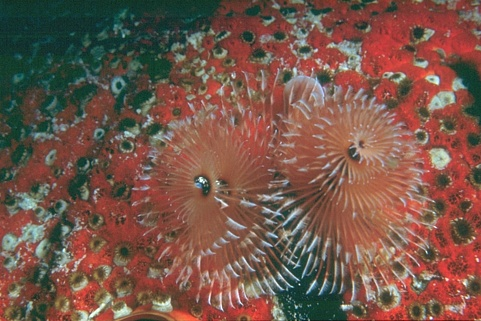
\includegraphics[width=73mm]{fig/Imagen3.jpg}}
%		\subfigure[Imagen Mejorada]{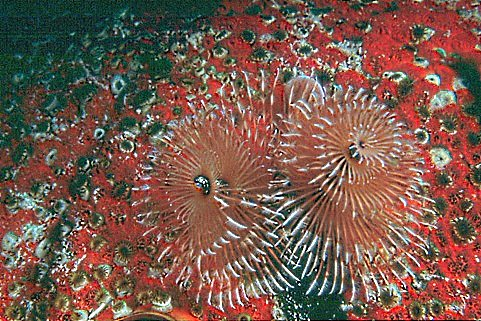
\includegraphics[width=73mm]{fig/Resultado3_3_4.jpg}}
%		  \caption{(a) Imagen con mejora de contraste aplicando 4 veces la ecuación \ref{contraste} con el método de ordenamiento propuesto}
%  \label{fig:mejora}
%\end{figure}

\begin{figure}
	\makebox[\linewidth][c]{%
		\begin{subfigure}[b]{0.5\textwidth}
			\centering
			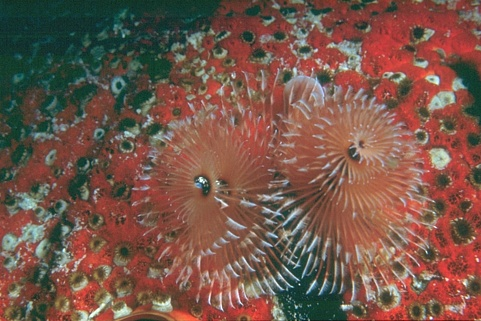
\includegraphics[width=0.8\textwidth]{fig/Imagen3.jpg}
			\caption{Original image}
			\label{fig:imagen_original_3}
		\end{subfigure}
	}\\
	\makebox[\linewidth][c]{%
		\begin{subfigure}[b]{0.5\textwidth}
			\centering
			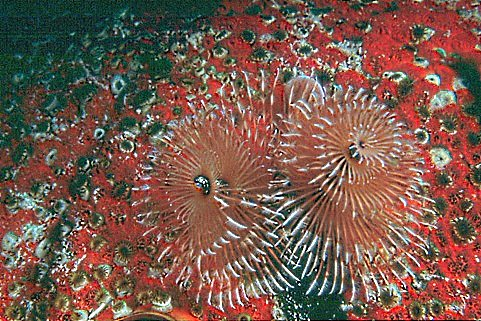
\includegraphics[width=0.8\textwidth]{fig/Resultado3_3_4.jpg}
			\caption{Improved image}
			\label{fig:imagen_mejorada_3}
		\end{subfigure}
	}\\
	\caption{(a) Image contrast improvement applying 4 times the equation \ref{contraste} with the proposed sorting method}
  \label{fig:mejora}
\end{figure}


\subsection{Application 3: Classification of textures}

 The problem of texture characterization and classification consists of two steps. In the first instance, image characteristics that allow numerically describe their textural properties using a feature vector or descriptor are calculated. Later it is assigned a class of texture according criteria of similarity between descriptors \cite{hanbury2005illumination}.

The granulometry and morphological covariance are the main morphological tools of texture characterization, both used intensity distributions to describe the properties of the textures \cite{lefevre2009beyond}.

%Los descriptores de textura morfológicos tienen la capacidad de describir efectivamente la regularidad y la direccionalidad por medio de la granulometría y la covarianza morfológica  \cite{hanbury2005illumination}. 

The way the color and texture information is incorporated into the descriptor is studied in \cite{palm2004color,van2005parallel}. In this work the morphological tools use the integrative approach where color and texture information are processed together.

The granulometry  was proposed in \cite{matheron1975random}  and is applied in feature extraction and estimation of size \cite{vincent2000granulometries,soille2013morphological}. Consists of a  $f \,\circ \, \lambda B $ openings family of $n+1$ elements including the input image. It is parameterized by the growing  $\lambda$ size of the structural element  ($0 \leq \lambda \leq n $). The values are collected by an evaluation measure that is usually the volume ($\mathrm{Vol}$):

\begin{equation}
G^{n}_{j}(f,\lambda)= \mathrm{Vol}([f\circ \lambda B ]_{j}) \; / \; \mathrm{Vol}(f_{j})
\end{equation}

Where $j$ is the j-th component of the color image $f$ and the volume is defined as:
\begin{equation}
\mathrm{Vol}(f_j) = \sum_{\substack{u\in \{1, ..., M\}\\ v \in \{1, ..., N\}}}[f(u,v)]_{j} 
\end{equation}

The morphological covariance proposal at \cite{matheron1975random,maragos1989pattern} denoted by  $K$ of $f$ image, is defined as the volume of the image $f$, after applying $\varepsilon$  erosion from a pair of pixels $(u,v)$ and  $(u',v')$ separated by a vector $\vec{v}$ denoted by  $P_{2,\vec{v}}$.\\
In practice $K $ is calculated by applying $\varepsilon$ erosion  to the original image $f$ with the structuring element $P_{2,\vec{v}}$ varying orientations and lengths of $\vec{v}$, where $n$ is the number of variations of $\vec{v}$. Its normalized version is given by:
\begin{equation}
K^{n}_{j}(f,P_{2,\vec{v}})  = \mathrm{Vol}([\varepsilon(f,P_{2,\vec{v}})]_{j}) / \mathrm{Vol}(f_{j})
\end{equation}
Allows to obtain a distribution of orientation and distance from a texture image \cite{aptoula2007morphological}.

The sorting method used to support the morphological characterization tools of texture, affects the percentages of classification. This is because the intensity distributions used as texture descriptors, vary according to the intermediate images. These intermediate images are the result of applying a morphological filter.

%--------------------------------------------------------
\subsubsection{Results}
\label{sec:resultadosexperi}
The tests were made with OutexTC13 data base consisting of 1360 images of size  128 $\times $ 128 pixels, with 68 kinds of surface textures (Figura \ref{fig:outex13} with 20 samples of each class, where the 50\% of each class is the training set. Totaling 680 training and test images respectively \cite{ojala2002outex}.  
The classifier used was k-nn (k-nearest neighbors) using Euclidean distance with k = 1. 

\begin{figure}
	\centering
		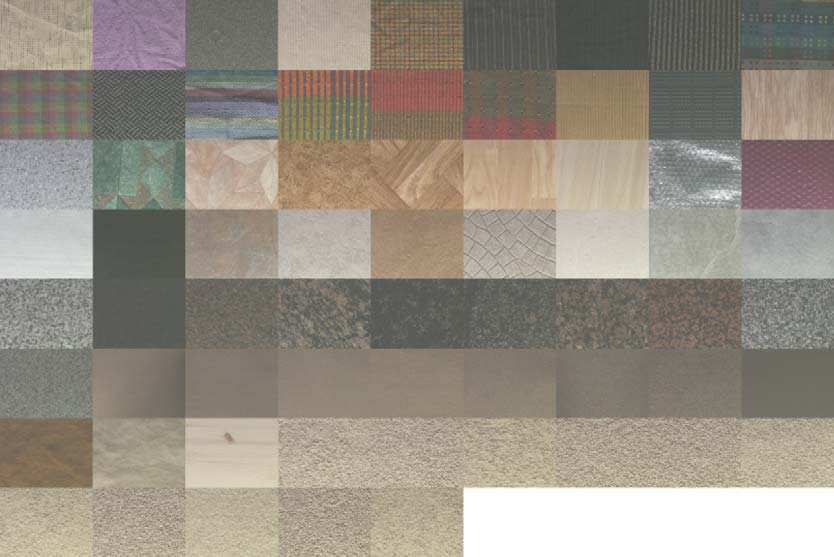
\includegraphics[scale=0.25]{fig/outex13.png}
	\caption{Texture samples OutexTC13}
	\label{fig:outex13}
\end{figure}

The purpose of the experiment was the classification percentages obtained using the sorting methods exposed.
Several statistical parameters were evaluated in the order strategy proposed in this work.
%---configuracion de la granulometria
In granulometry tests they have been used structural elements of square shape of size  $\lambda$ and $2\lambda+1$ side pixels, varying $\lambda$ from 1 to 15. For each element of the series, 15 values for each channel are calculated which are then concatenated. The choice of simple increase of $\lambda$, is based on the smallest increases provide better classification results \cite{de2006selecting}. 
With respect to the configuration of the parameters of the proposal, each texture sample was divided in $2\times2$  subregions and  denoted by the suffix W4. This division allows each texture sample is divided equally and perceptually similar. Is denoted by the suffix B when the image domain is the structuring element itself. 

%---configuracion de la covarianza morfologica
Morphological covariance requires varying the direction and distance between the pair of points that composing the structural elemen. The addresses used were $0^{\circ}$, $45^{\circ}$, $90^{\circ}$,  $135^{\circ}$, in practice only these addresses are important and significantly recognizable \cite{hanbury2005illumination}. The separation distances were used for each direction were from 1 a 20 píxeles. Using these 4 directions and 20 distances have generated 80 values for each channel, finally these values are concatenated to obtain the feature vector of the texture sample. 
 
\begin{table}
\caption{Classification results by Ordering Methods}
\label{tab:experiment1_t1}

\begin{tabular}{@{}lrr@{}}
\toprule
&\multicolumn{2}{c}{ \% 
Correctly classified }\\
\cline{2-3}
\textbf{Sort } & \textbf{Covariance} &\textbf{Granulometry } \\ 
\cmidrule{1-3}
%Marginal  & 85,78 & 88,68 \\ \hline
BM & 79,56 & 77,79 \\ \hline
ED & 81,91 & \textbf{84,11}  \\ \hline
LEX & 79,74 & 80,15 \\ \hline
ALEX & 76,32   &  69,12  \\ \hline
AMLEX &  81,62   &  81,30  \\ \hline
HLEX &  \textbf{83,97}  &  77,35  \\ \hline
DLAB  & \textbf{84,26}  & 72,35   \\ \hline
MEANW4 & 81,47 & 78,97 \\ \hline %$\mathrm{HST_{2}} $ Promedio 
%$\mathrm{HST_{2}} $ Entropía & 82,65 & \textbf{85,88} \\ \hline
SMOW4 & 82,50 & \textbf{85,44} \\ \hline %$\mathrm{HST_{2}} $
MO1W4 & 81,76 & 82,65 \\ \hline %$\mathrm{HST_{2}} $ Moda Min  
MO2W4 & 80,44 & 80,01 \\ \hline %$\mathrm{HST_{2}} $ Moda Max  
MAXW4 & 81,62 & 81,32 \\ \hline % $\mathrm{HST_{2}} $ Máximo
MINW4 & 81,47 & 83,38 \\ \hline %$\mathrm{HST_{2}} $ Mínimo 
VAR   & 81,76 &  83,97  \\ \hline 
MEANB & 81,91 & 78,82 \\ \hline %$\mathrm{HST}_{ b} $ Promedio
SMOB & \textbf{83,82} & \textbf{84,71} \\ \hline %$\mathrm{HST}_{b} $ Suavidad
MO1B & 82,01  & 83,23  \\ \hline %$\mathrm{HST_{2}} $ Moda Min  
MO2B & 81,21 &  81,36  \\ \hline %$\mathrm{HST_{2}} $ Moda Max  
MAXB & 81,32 & 81,06 \\ \hline %$\mathrm{HST}_{ b} $ 
MINB & 81,05 & 83,12 \\ \hline %$\mathrm{HST}_{ b} $
VARB & 83,09 &  82,21  \\ \hline 
%$\mathrm{HST_{2}} $ Desviación  & 82,01 & \textbf{85,02} \\ \hline
%$\mathrm{HST_{2}} $ Asimetria  & 81,91 & 83,09 \\ \hline
%$\mathrm{HST_{2}} $ Uniformidad & 80,74 & 80,44 \\ \hline
%$\mathrm{HST_{2}} $ Momento muestral & 79,56 & 60,88 \\ \hline
%$\mathrm{HST}_{ b} $ Desviación & \textbf{82,94} & \textbf{85,29} \\ \hline
%$\mathrm{HST}_{ b} $ Asimetría & \textbf{83,24} & \textbf{84,85} \\ \hline
%$\mathrm{HST_{2}} $ Energía & 82,35 & 79,56 \\ \hline
%$\mathrm{HST}_{ b} $ Entropía & 82,21 & 64,85 \\ \hline
%$\mathrm{HST}_{ b} $ Uniformidad & 80,59 & 80,29 \\ \hline
%$\mathrm{HST}_{ b} $ Momento Muestral & 46,47 & 62,78 \\ \hline
%$\mathrm{HST}_{ b} $ Energía & 82,03 & 81,47 \\ \hline
%$\mathrm{HST}_{ 2,4,8} $ Promedio & 81,62 & 84,12 \\ \hline
%$\mathrm{HST}_{ 2,4,8} $ Entropia & 82,79 & \textbf{85,74} \\ \hline
%$\mathrm{HST}_{ 2,4,8} $ Asimetría & 81,91 & 82,65 \\ \hline
%$\mathrm{HST}_{ 2,4,8} $ Desviación & 82,50 & 84,41 \\ \hline
%$\mathrm{HST}_{ 2,4,8} $ Uniformidad  & 80,74 & 80,59 \\ \hline
%$\mathrm{HST}_{ 2,4,8} $ Suavidad  & 82,50 & 84,56 \\ \hline
%$\mathrm{HST}_{ 2,4,8} $ Momento Muestral & 79,12 & 60,88 \\ \hline
%$\mathrm{HST}_{ 2,4,8} $ Moda  & 81,76 & 83,09 \\ \hline
%$\mathrm{HST}_{ 2,4,8} $ Máximo & 81,62 & 81,32 \\ \hline
%$\mathrm{HST}_{ 2,4,8} $ Mínimo & 81,47 & 83,53 \\ \hline
%$\mathrm{HST}_{ 2,4,8} $ Energía & 82,35 & 75,88 \\ \hline
\end{tabular}
\label{exper_ordenaciones}
\end{table}
%-  - - - - - - - - - - - - - -
In the Table \ref{tab:experiment1_t1} the three best results of each method were marked in bold. Covariance Morphological with HLEX y DLAB orderings have higher performances of $\approx 1\%$ with respect to SMOW4 that presented the best performance in RGB space. The results are consistent with experiments in \cite{hanbury2005illumination} where best results are obtained in the L*a*b space compared to RGB space using structuring elements of variant length. This is because in those color spaces the chromatic information is separated of the brightness or intensity. 
In experiments mentioned in \cite{bianconi2011theoretical} about the perception of texture they indicate that the texture and color are perceived independently. 
With the granulometry, the RGB space has better results with SMOW4 and SMOB orderings, both higher than the ED ordering at ($\approx 1,33 \% $). Moreover, the ED ordering provides far superior results to the BM, LEX, ALEX and AMLEX orderings.

The SMOW4 y SMOB orderings (85,44\%, 84,71\%) show the best results of classification (with granulometry) with respect to the ordering methods implemented of the state of the art. The division in $2\times2$ sub-regions (W4) leads to better results than using B.  

\section{Conclusions and Future Work}

In this work a new strategy of RGB color ordering that is dependent on the image we are presented. The ordering is performed by extracting histogram information of each color component in a certain domain image. Two strategies of domain decomposition are presented to extract this information, one is extracting information from the same window filter, and another consists in dividing the image into sub-regions of same size, taking the union of them when the filter window takes more than one sub-region.
Tests were performed for three image processing applications: Noise Removal, contrast stretching and textures characterization for further classification. Is used morphologythis mathematical for this two latest applications. Morphological operators in this case are pseudo-operators as it can not be guaranteed certain theoretical properties, such as idempotency. 
The median filter was used to eliminate noise, achieving better results with some extracted weights of different methods of the state of the art, both gaussian noise such as speckle. For salt and pepper noise the euclidean distance to the origin in the RGB color space in the MAE metric gave better results than the proposed method  with the different extracted information for each component. This is because the salt noise is expressed by the minimum value in each color component, and pepper noise is expressed as the maximum value in each component. Thus, if the colors of the pixels are sorted by the euclidean distance, it is quite unlikely that the median filter select a pixel to be noise. 
For the application of contrast improvement the proposed method was more efficient according to the CEF metric with different weights extracted from image information. For the characterization of textures using Covariance Morphological with lexicographic ordering I→H→S \cite{ortiz2004gaussian} and the euclidean distance to the color $(0,0,0)$ in the L*a*b* color space \cite{ortiz2002procesamiento} has better performance to the proposal, demonstrated in its best ranking. The proposed method using the softness as weight for each component achieves better results using the granulometry as characterization of textures.
Is proposed as future work analyze the importance of domain decomposition to extract information from each color component. More experiments could be done in different applications such as fusion or segmentation of color image. Could be extract other information for each component as Entropy and Energy.
 


%Por lo tanto en $K^{TH}$, el contraste  entre las \'areas brillantes y oscuras de la imagen $f$ es mayor.

%En la actualidad existen varios operadores de contraste compuestos y multiescala a partir de la transformada top-hat \cite{bai2012toggle}. Como el objetivo de este trabajo no es crear un nuevo operador de contraste sino validar la estrategia de ordenamiento de color  usaremos la ecuaci\'on \ref{contraste} en la aplicaci\'on de mejoramiento de contraste. Con la misma se podr\'a comparar los diferentes trabajos del estado de arte y la propuesta en la secci\'on de experimentos.

%\section{Section title}
%\label{sec:1}
%Citation of \cite{trouiller2002drug}.
%\subsection{Subsection title}
%\label{sec:2}
%as required. Don't forget to give each section
%and subsection a unique label (see Sect.~\ref{sec:1}).
%\paragraph{Paragraph headings} Use paragraph headings as needed.
%\begin{equation}
%a^2+b^2=c^2
%\end{equation}

% For one-column wide figures use
%\begin{figure}
%\centering
% Use the relevant command to insert your figure file.
% For example, with the graphicx package use
%  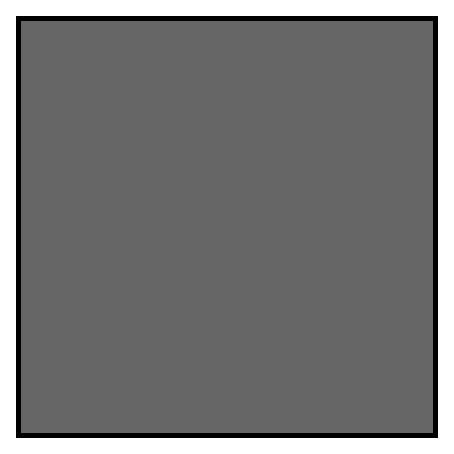
\includegraphics{example.eps}
% figure caption is below the figure
%\caption{Please write your figure caption here}
%\label{fig:1}       % Give a unique label
%\end{figure}
%
% For two-column wide figures use
%\begin{figure}
%\centering
% Use the relevant command to insert your figure file.
% For example, with the graphicx package use
%  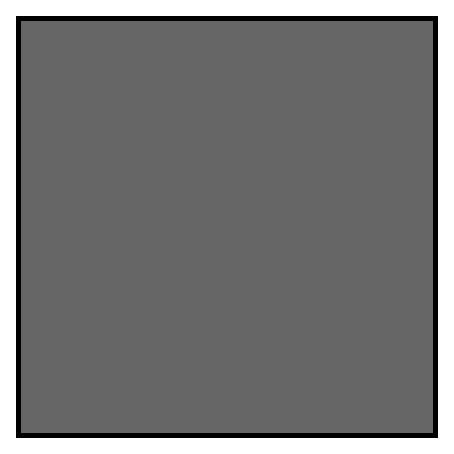
\includegraphics[width=0.75\textwidth]{example.eps}
% figure caption is below the figure
%\caption{Please write your figure caption here}
%\label{fig:2}       % Give a unique label
%\end{figure}
%
% For tables use
%\begin{table}[h]
% table caption is above the table
%\caption{Please write your table caption here}
%\centering
%\label{tab:1}       % Give a unique label
% For LaTeX tables use
%\begin{tabular}{lll}
%\hline\noalign{\smallskip}
%first & second & third  \\
%\noalign{\smallskip}\hline\noalign{\smallskip}
%number & number & number \\
%number & number & number \\
%\noalign{\smallskip}\hline
%\end{tabular}
%\end{table}


%\begin{acknowledgements}
%If you'd like to thank anyone, place your comments here
%and remove the percent signs.
%\end{acknowledgements}

% BibTeX users please use
\bibliographystyle{spbasic}
\bibliography{sample}   % name your BibTeX data base

% Non-BibTeX users please use
%\begin{thebibliography}{}
%
% and use \bibitem to create references. Consult the Instructions
% for authors for reference list style.
%
% Format for Journal Reference
%\bibitem[Author I(1999)]{RefJ}
%Author I (year) Article title. Journal Title-Abbreviated Vol: pp--pp
% Format for books
%\bibitem[Author and Smith(2001)]{RefB}
%Author I, Smith J (year) Book title. Publisher, Place, pp numbers
% etc
%\end{thebibliography}

\end{document}
% end of file template.tex
